\documentclass{article}

%%%%%%%%%%%%%%%%%%%%%%%%%%%%%%%%%%%%%%%%%%%%%%%%%%%%%%%%%%%%%%%%%%%%%%%%%%%
%%%%%%%%%%%%%%%%%%%%%%% Page Layout and Typography %%%%%%%%%%%%%%%%%%%%%%%
%%%%%%%%%%%%%%%%%%%%%%%%%%%%%%%%%%%%%%%%%%%%%%%%%%%%%%%%%%%%%%%%%%%%%%%%%%%

\usepackage[utf8]{inputenc}
\usepackage{geometry}
\usepackage{indentfirst}
\usepackage{parskip}
\usepackage{pslatex}
\usepackage{setspace}
\geometry{
    left=1in,
    right=1in,
    top=0.8in,
    bottom=0.8in,
}


%%%%%%%%%%%%%%%%%%%%%%%%%%%%%%%%%%%%%%%%%%%%%%%%%%%%%%%%%%%%%%%%%%%%%%%%%%%
%%%%%%%%%%%%%%%%%%%%%%%% Figures, Captions, and Lists %%%%%%%%%%%%%%%%%%%%%
%%%%%%%%%%%%%%%%%%%%%%%%%%%%%%%%%%%%%%%%%%%%%%%%%%%%%%%%%%%%%%%%%%%%%%%%%%%

\usepackage{graphicx}
\usepackage{float}
\usepackage[font=small, labelfont=bf]{caption}
\usepackage{subcaption}
\usepackage{enumitem} % set configuration for list
\usepackage{tabularx}
\usepackage{array}



%%%%%%%%%%%%%%%%%%%%%%%%%%%%%%%%%%%%%%%%%%%%%%%%%%%%%%%%%%%%%%%%%%%%%%%%%%%
%%%%%%%%%%%%%%%%%%%%%%%%%%%% Math Packages %%%%%%%%%%%%%%%%%%%%%%%%%%%%%%%%
%%%%%%%%%%%%%%%%%%%%%%%%%%%%%%%%%%%%%%%%%%%%%%%%%%%%%%%%%%%%%%%%%%%%%%%%%%%

\usepackage{amsmath,amsthm,amssymb}
\usepackage{mathtools}
\usepackage{bm}
\usepackage{dsfont}
\usepackage{arydshln} % dashed group boundaries in ANOVA design matrices


%%%%%%%%%%%%%%%%%%%%%%%%%%%%%%%%%%%%%%%%%%%%%%%%%%%%%%%%%%%%%%%%%%%%%%%%%%%
%%%%%%%%%%%%%%%%%%%%%%%%%%%% Title Helpers %%%%%%%%%%%%%%%%%%%%%%%%%%%%%%%%
%%%%%%%%%%%%%%%%%%%%%%%%%%%%%%%%%%%%%%%%%%%%%%%%%%%%%%%%%%%%%%%%%%%%%%%%%%%

\usepackage{titling}
\newcommand{\subtitle}[1]{
  \posttitle{
    \par\end{center}
    \begin{center}\large#1\end{center}\vspace{-3.5em}
    \vskip0.5em}
}


%%%%%%%%%%%%%%%%%%%%%%%%%%%%%%%%%%%%%%%%%%%%%%%%%%%%%%%%%%%%%%%%%%%%%%%%%%%
%%%%%%%%%%%%%%%%%%%%%%%%%%%%%%%% Colors %%%%%%%%%%%%%%%%%%%%%%%%%%%%%%%%%%%
%%%%%%%%%%%%%%%%%%%%%%%%%%%%%%%%%%%%%%%%%%%%%%%%%%%%%%%%%%%%%%%%%%%%%%%%%%%

\usepackage{xcolor}
\newcommand{\red}{\textcolor{red}}
\newcommand{\blue}{\textcolor{blue}}
\newcommand{\green}{\textcolor{green}}


%%%%%%%%%%%%%%%%%%%%%%%%%%%%%%%%%%%%%%%%%%%%%%%%%%%%%%%%%%%%%%%%%%%%%%%%%%%
%%%%%%%%%%%%%%%%%%%%%%%%%%%% Framed Blocks %%%%%%%%%%%%%%%%%%%%%%%%%%%%%%%%
%%%%%%%%%%%%%%%%%%%%%%%%%%%%%%%%%%%%%%%%%%%%%%%%%%%%%%%%%%%%%%%%%%%%%%%%%%%

% colored block, credit to Kevin Z. Lin
\definecolor{col0}{rgb}{0.950,0.930,0.855} %gray/beige
\usepackage{mdframed}
\newenvironment{block}
{	\begin{center}
    \vspace{1em}
   	\begin{mdframed}[
    backgroundcolor=col0,
    topline=false,
    bottomline=false,
    rightline=false,
    leftline=false,
    skipabove=20pt,  % space before
    skipbelow=20pt   % space after
    ]
}
{
   	\end{mdframed} 
   	\end{center}
}

% boxed text
\newenvironment{mybox}{%
  \par\addvspace{10pt}% space that survives right after \section
  \begin{mdframed}[skipabove=0pt,skipbelow=10pt]%
}{%
  \end{mdframed}%
}


%%%%%%%%%%%%%%%%%%%%%%%%%%%%%%%%%%%%%%%%%%%%%%%%%%%%%%%%%%%%%%%%%%%%%%%%%%%
%%%%%%%%%%%%%%%%%%%%%%%%% Theorem Environments %%%%%%%%%%%%%%%%%%%%%%%%%%%
%%%%%%%%%%%%%%%%%%%%%%%%%%%%%%%%%%%%%%%%%%%%%%%%%%%%%%%%%%%%%%%%%%%%%%%%%%%

% Define a custom theorem style that places the title on a separate line
\newtheoremstyle{break}
  {\topsep}   % Space above
  {\topsep}   % Space below
  {\itshape}  % Body font
  {}          % Indent amount
  {\bfseries} % Theorem head font
  {.}         % Punctuation after theorem head
  {\newline}  % Space after theorem head (THIS IS THE LINEBREAK)
  {}          % Theorem head spec

% Apply this style and define 'Fact'
\theoremstyle{break}


%%%%%%%%%%%%%%%%%%%%%%%%%%%%%%%%%%%%%%%%%%%%%%%%%%%%%%%%%%%%%%%%%%%%%%%%%%%
%%%%%%%%%%%%%%%%%%%%%%%%%%%%%%%%% Links %%%%%%%%%%%%%%%%%%%%%%%%%%%%%%%%%%%
%%%%%%%%%%%%%%%%%%%%%%%%%%%%%%%%%%%%%%%%%%%%%%%%%%%%%%%%%%%%%%%%%%%%%%%%%%%

\usepackage[colorlinks=true,
            linkcolor=blue,
            urlcolor=blue,
            citecolor=blue]{hyperref}


%%%%%%%%%%%%%%%%%%%%%%%%%%%%%%%%%%%%%%%%%%%%%%%%%%%%%%%%%%%%%%%%%%%%%%%%%%%
%%%%%%%%%%%%%%%%%%%%%%%%%%%%%%%% Notation %%%%%%%%%%%%%%%%%%%%%%%%%%%%%%%%%
%%%%%%%%%%%%%%%%%%%%%%%%%%%%%%%%%%%%%%%%%%%%%%%%%%%%%%%%%%%%%%%%%%%%%%%%%%%
% Number systems and common spaces
\newcommand{\R}{\ensuremath{\mathbb{R}}}
\newcommand{\Z}{\ensuremath{\mathbb{Z}}}
\newcommand{\N}{\ensuremath{\mathbb{N}}}
\newcommand{\E}{\ensuremath{\mathbb{E}}}
\newcommand{\F}{\ensuremath{\mathcal{F}}}

% Bold random vectors / matrices
\newcommand{\bX}{\ensuremath{\mathbf{X}}}
\newcommand{\bY}{\ensuremath{\mathbf{Y}}}
\newcommand{\bZ}{\ensuremath{\mathbf{Z}}}

% Basic math shortcuts
\newcommand{\st}{\ensuremath{\text{ s.t. }}}
\newcommand{\dd}{\ensuremath{\mathrm{d}}}

% Delimiters
\newcommand{\p}[1]{\ensuremath{\left(#1\right)}}
\newcommand{\br}[1]{\ensuremath{\left\{#1\right\}}}
\newcommand{\sbr}[1]{\ensuremath{\left[#1\right]}}
\newcommand{\abs}[1]{\ensuremath{\left|#1\right|}}
\newcommand{\norm}[1]{\ensuremath{\left\lVert#1\right\rVert}}
\newcommand{\ip}[1]{\ensuremath{\left\langle #1 \right\rangle}}
\newcommand{\ceil}[1]{\ensuremath{\left\lceil#1\right\rceil}}
\newcommand{\floor}[1]{\ensuremath{\left\lfloor#1\right\rfloor}}

% Probability and statistics
\newcommand{\Prob}[2]{\ensuremath{\mathbb{P}_{#1}\left(#2\right)}}
\newcommand{\Ind}[2]{\ensuremath{\mathds{1}_{#1}\left(#2\right)}}
\newcommand{\iid}{\ensuremath{\mathrm{i.i.d.}}}
\newcommand{\iidsim}{\ensuremath{\overset{\mathrm{i.i.d.}}{\sim}}}
\newcommand{\cdf}{\ensuremath{\mathrm{c.d.f.}}}
\newcommand{\pdf}{\ensuremath{\mathrm{p.d.f.}}}
\newcommand{\pmf}{\ensuremath{\mathrm{p.m.f.}}}
\DeclareMathOperator{\Var}{Var}
\DeclareMathOperator{\Cov}{Cov}
\DeclareMathOperator{\Bernoulli}{Bernoulli}
\DeclareMathOperator{\Binomial}{Binomial}
\DeclareMathOperator{\Geometric}{Geometric}
\DeclareMathOperator{\Multinomial}{Multinomial}
\DeclareMathOperator{\NegativeBinomial}{NegativeBinomial}

% Linear algebra and geometry
\DeclareMathOperator{\Row}{Row}
\DeclareMathOperator{\tr}{tr}
\DeclareMathOperator{\Span}{Span}
\DeclareMathOperator{\diag}{diag}
\DeclareMathOperator{\rank}{rank}
\DeclareMathOperator{\conv}{conv}
\DeclareMathOperator{\aff}{aff}
\newcommand{\op}{\ensuremath{\mathrm{op}}}

% Optimization
\DeclareMathOperator*{\argmax}{arg\,max}
\DeclareMathOperator*{\argmin}{arg\,min}


%%%%%%%%%%%%%%%%%%%%%%%%%%%%%%%%%%%%%%%%%%%%%%%%%%%%%%%%%%%%%%%%%%%%%%%%%%%
%%%%%%%%%%%%%%%%%%%%%%%%%% Document begins here %%%%%%%%%%%%%%%%%%%%%%%%%%%
%%%%%%%%%%%%%%%%%%%%%%%%%%%%%%%%%%%%%%%%%%%%%%%%%%%%%%%%%%%%%%%%%%%%%%%%%%%

\author{Wenbin Wu}
\title{BIOS762 Review}


\begin{document}
\maketitle


% Paragraph 1: role of these notes
The following notes are based on the lecture slides of BIOS762 (Linear Models) at UNC Chapel Hill. They are compiled from the author's \emph{personal understanding} of the course material and aim to summarize the key results, highlight connections among the main concepts and theorems, and collect useful problem-solving strategies.

% Paragraph 2: suggested use
These notes are \emph{not} intended to be a comprehensive summary of the lecture slides, but rather a supplementary resource. They are most useful as a review document after a first pass through the lecture slides or as a quick reference while working through exam problems.

For simplicity, some notation differs from that used in the lecture slides. If any statement is unclear or appears incorrect, please verify it against the course materials and consult other reliable references. We also encourage the use of AI assistants together with these notes and the relevant course materials to clarify concepts, fill in omitted details, and answer questions that arise while studying.

% Paragraph 3: acknowledgment and contributions
We thank Dr. Ethan Alt for sharing his abridged BIOS762 notes through the GitLab student repository, portions of which have been adapted in this document. 
We warmly welcome corrections, suggestions, and contributions from readers. 
If you would like to contribute, please submit a pull request through the GitHub repository: \url{https://github.com/WenbinWu2001/oh-my-qualify-theory}.

\tableofcontents
\newpage

\section{Preliminaries for linear model}\label{sec:prelim-lm}
This section presents the basic mathematical tools used to derive the main results for linear models. The main results are covered in Slides pp. 24-113, 124, 176-185, and we also include some additional results that are useful in practice.

\subsection{Column spaces}\label{sec:prelim-lm-column-spaces}
Notation: 
We use $A \in C(X)$ to denote that all columns of $A$ belong to $C(X)$. 
We write $A \oplus B$ for the direct sum of two orthogonal subspaces $A$ and $B$.


\subsubsection{Basic facts}
Let $A \in \R^{m \times n}$ be a general matrix.
\begin{align*}
    & C(A) = N(A')^\perp\\
    & C(A) = C(AA'), \qquad N(A) = N(A'A), \qquad \Row(A) = \Row(A'A)\\
    & C(A'A) = \Row(A'A), \qquad C(AA') = \Row(AA')\\
    & r(A') = r(A) = r(A A') = r(A'A)\\
    & \rank(A) + \mathrm{nullity}(A) = n \\
    & v \in C(A) \ \Leftrightarrow\ \exists\ w\in\R^n \st v = Aw.
\end{align*}

\subsubsection{Post-multiplicate $A$ by $B$ preserves or reduces $C(A)$.}
Suppose $A \in \R^{n \times p},\ B \in \R^{p \times s}$ and $r(A) = r \leq \min(n,p)$, then
\begin{itemize}
    \item In general, $C(AB) \subset C(A), \quad N(B) \subset N(AB)$.
    \item If $r(AB) = r$ (i.e., the rank of $A$ remains unchanged), then $C(A) = C(AB)$ and we say that $B$ is rank-preserving. A sufficient condition is $C(B) \supset N(A)^\perp$.
    \item If $B$ is a square nonsingular matrix, then $C(A) = C(AB)$.
\end{itemize}

\subsubsection{Pre-multiplicate $B$ by $A$ preserves or reduces $\Row(A)$.}

(This result is not important for this course though.)

Suppose $A\in\mathbb R^{n\times p}$ and $B\in\mathbb R^{p\times s}$. Pre-multiplication can only preserve or reduce the row space: $\Row(AB)\subseteq \Row(B)$.
\[
\rank(AB)=\rank(B)
\quad\Leftrightarrow\quad
N(A)\cap C(B)=\{0\}.
% --- DO NOT DELETE ---
% \footnote{
%     To prove this, observe that $C(AB)=A\bigl(C(B)\bigr)$.
%     Consider the restriction
%     $A|_{C(B)}:C(B)\longrightarrow \mathbb R^n$.
%     Its kernel is $\ker\left(A|_{C(B)}\right)=N(A)\cap C(B)$.\\
%     Apply rank-nullity theorem, we obtain
%     \[
%     \rank(AB) 
%     = \dim A(C(B)) 
%     = \dim C(B)-\dim\bigl(N(A)\cap C(B)\bigr)
%     = \rank(B)-\dim\bigl(N(A)\cap C(B)\bigr).
%     \]
%     Therefore,
%     \[ 
%     \rank(AB)=\rank(B) 
%     \Longleftrightarrow \dim\bigl(N(A)\cap C(B)\bigr)=0
%     \Longleftrightarrow N(A)\cap C(B)=\{0_n\}.
%     \]
% }
\]

\subsubsection{Orthogonal complement of a column space}
Given $X \in \R^{n\times p}$, how do we find the orthogonal complement of its column space $C(X)^\perp$?

\textbf{Method 1:} 
$C(X)^\perp = N(X')$, where the latter is found by solving $X'v = 0$.\\
\textbf{Method 2:} 
Apply Gram-Schmidt to the columns of $X$ to obtain an orthonormal basis $\{q_1,\ldots,q_r\}$ for $C(X)$, and then extend it to an orthonormal basis $\{q_1,\ldots,q_n\}$ for $\R^n$. The remaining vectors $\{q_{r+1},\ldots,q_n\}$ form an orthonormal basis for $C(X)^\perp$.


\subsection{Matrix decomposition}\label{sec:prelim-lm-matrix-decomp}
\textbf{Importance:} SVD $>$ QR $>$ Spectral.

\textbf{Commonly used result (from Spectral decomposition):}\\
Let $A \in \R^{n \times n}$, then
\begin{align*}
    A \text{ is PSD} \quad &\Longleftrightarrow \quad \exists\ Q\in \R^{n \times n} \text{with orthogonal columns such that } A = QQ' \text{ with } r(A) = r(Q).\\
    A \text{ is PD} \quad &\Longleftrightarrow \quad \exists \text{ nonsingular } Q\in \R^{n \times n} \text{with orthogonal columns such that } A = QQ'.
\end{align*}
Here, $Q=U\Lambda^{1/2}$ is constructed from the spectral decomposition $A=U\Lambda U'$.



\subsection{Generalized inverse}\label{sec:prelim-lm-g-inverse}
Suppose $A \in \R^{n \times p}$ (take $A = X$ in a linear model). 
We use ``g-inverse'' as shorthand for ``generalized inverse''.
\begin{itemize}
    \item Def: $A^- \in \R^{p \times n}$ is a g-inverse of $A$ if $AA^- A = A$. 
    \item Def: $A^+ \in \R^{p \times n}$ is the (unique) MP g-inverse of $A$ if (1) both $AA^+$ and $A^+ A$ are symmetric, and (2) $A^+$ and $A$ are the g-inverse of each other.
    \item $A^+$ can be constructed from the compact SVD. Let $A = V_1 \Delta U_1'$, then $A^+ = U_1 \Delta^{-1} V_1'$.
    \item $A^+ = (A'A)^{-1}A'$ when $A$ has full column rank. 
    \footnote{For the OLS problem, when $X$ has full column rank, $\hat{\beta}_{\mathrm{OLS}} = X^+ Y = (X'X)^{-1} X'Y$.}
    In this case, $A^+ A = (A'A)^{-1}A'A = I_p.$
    \item MP g-inverse and g-inverse always exist for any matrix.
    \item Similar to the regular inverse: for any matrix $A$, (1) $(A^+)' = (A')^+$, (2) $(A^+)^+ = A$, (3) If $A$ is symmetric, then $A^+$ is also symmetric. However, $(AB)^+ \neq B^+ A^+$ in general. 
    \footnote{Special cases when $(AB)^+ = B^+ A^+$ holds: (1) when $A$ and $B$ are both nonsingular; (2) for any $A$, $(A'A)^+ = A^+(A')^+$; (3) when $A$ has full column rank $p$ and $B$ has full row rank $p$.}
    \item $C(A^+) = C(A')$, $\rank(A^+) = \rank(A)$.
    \item $AA^-$ is a projection onto $C(A)$. $AA^+$ is the o.p.o. onto $C(A)$.
    \item $A^- A$ is a projection onto some subspace of $C(A^-)$. $A^+ A$ is the o.p.o. onto $C(A^+) = C(A')$.
\end{itemize}


\subsection{Projection}\label{sec:prelim-lm-projection}
We use ``o.p.o.'' as shorthand for ``orthogonal projection operator''.

\subsubsection{Basic facts}
Suppose $X \in \R^{n \times p}$.
\begin{itemize}
    \item If $M$ is the o.p.o. onto $C(X)$, then $M$ is unique and $C(M) = C(X)$. Moreover, $I-M$ is the unique o.p.o. onto $C(X)^\perp$.
    \item In a linear model $Y = X\beta + \epsilon$, we have $M = X (X'X)^{-1} X'$ when $X$ is full-rank. When $X$ is not full-rank, we have $M = X X^+ = X (X'X)^- X'$ (the latter is invariant to the choice of g-inverse).
    \item The o.p.o. to $N(X) = C(X')^\perp$ is $P = I_p - M_{X'}$ where $M_{X'} = X' (X')^+ = X'(XX')^- X \in \R^{p \times p}$. We can hence use $Pz,\ z\in \R^p$ to represent any vector in $N(X)$.
    \item Suppose $X$ is an $n \times p$ matrix of rank $r \leq \min(n,p)$. 
    Suppose $\{a_1, \ldots, a_r\}$ is an orthonormal basis for $C(X)$ (which can be found by decomposing $X$). Let $A = (a_1, \ldots, a_r)$, where $a_i$ is $n \times 1$. Then,
    \[AA' = \sum_{i=1}^r a_i a_i'\]
    is the unique o.p.o. onto $C(X)$.
    \item Given two o.p.o. $M$ and $M_0$, if $C(M_0) \subset C(M)$, then (1) $MM_0 = M_0M = M_0$, (2) $C(M_0) \perp C(M-M_0)$, (3) $M - M_0$ is the o.p.o. onto $C(M-M_0) = C(M) \cap C(M_0)^\perp$, i.e., the orthogonal complement of $C(M_0)$ relative to $C(M)$.
    \item \textit{The o.p.o. onto the sum of two \emph{orthogonal} subspaces is the sum of their o.p.o.'s.}\\
    Given two o.p.o. $M_1, M_2 \in \R^{n \times n}$, we have 
    \[
    M_1 + M_2 \text{ is the o.p.o. onto $C(M_1, M_2)$} 
    \quad\Leftrightarrow\quad 
    C(M_1) \perp C(M_2).
    \]
    Here, $$C(M_1) \perp C(M_2) \quad\Leftrightarrow\quad M_1 M_2 = 0.$$
    Note that the RHS implies $M_2 M_1 = M_2' M_1' = (M_1 M_2)' = 0$.
\end{itemize}

\subsubsection{Computing the o.p.o. onto $C(X)$}
Let $M \in \R^{n \times n}$ denote the o.p.o. onto $C(X)$.

\textbf{Method 1:} Form a full-rank $X^* \in \R^{n \times r}$ that contains the linearly independent columns of $X$ with $C(X^*) = C(X)$ (i.e., remove the redundant columns of $X$). Then $M = X^* (X^{*'} X^*)^{-1} X^{*'}$.\\
\textbf{Method 2:} Construct an orthonormal basis $Q$ of $C(X)$. 
This can be obtained by applying Gram-Schmidt to $X$, using the QR decomposition of $X$ (set $Q = Q_1$ in the QR),or using the SVD of $X$ (set $Q = V_1$ in the SVD). Then $M = QQ'$.\\
\textbf{Method 3:} $M = X X^+$, where $X^+$ is the MP g-inverse of $X$ obtained from the reduced SVD of $X$ (Slides pp. 88, 91).

\subsubsection{Proving projection}
Let $A \in \R^{n \times n}$. How do we show that $A$ is a projection operator onto $C(A)$ along $N(A)$?

\textbf{Method 1}: Prove by definition. Show that $\forall v \in C(A),\ Av = v$ and $\forall v\in N(A),\ Av=  0$. To show $A$ is an orthogonal projection, we show additionally that $N(A) = C(A)^\perp$ (or $\forall v \in C(A)^\perp, \ Av = 0$).\\
\textbf{Method 2}: Show that $A$ is idempotent, i.e., $A^2 = A$, then show ``onto'', i.e., the target subspace is $C(A)$. To show $A$ is an orthogonal projection, we show additionally that $A = A'$.

The orthogonal decomposition Theorem on Slides p. 46 is useful to prove propositions. That is, decompose $x = x_0 + x_1 \in \R^n$ with $x_0 \in C(A)$ and $x_1 \in C(A)^\perp$ (both are unique), and continue the proof.

\textbf{Remark:} The arguments above look obvious and trivial. But in the question, $A$, $C(A)$ and $N(A)$ could be replaced by specific matrices or spans of vectors, then you need to show each equation mentioned above by calculation. For example, if $A$ is already known to be a projection and $C(A)\subseteq C(X)$, then showing $AX=X$ establishes $C(X)\subseteq C(A)$ and hence proves that $A$ projects onto $C(X)$.


% --- nonessential, but don't delete ---
% \subsubsection{Find an oblique projection operator}
% \blue{Change of basis + $diag(1,1,\ldots, 1,0, 0,\ldots 0)$ to eliminate the along-subspace in the transformed basis. See bootcamp problems.}


\subsection{Quadratic form of a random vector}\label{sec:prelim-lm-quad-form}
The main results are covered in Slides pp. 176-185.

Suppose $Y$ is an $n$-dimensional random vector and let $A$ be an $n \times n$ matrix of constants. A quadratic form is a random variable defined by $Y'AY$ for some $Y$ and $A$.

\textbf{Theorem:} (Mean of a quadratic form.)\\
Let $Y$ be an $n \times 1$ random vector with $\E[Y] = \mu$ and $\Cov(Y) = \Sigma$, then
\[
\E[Y'AY] = \mu' A \mu + \tr(A\Sigma).
\]

\subsubsection{Distribution of quadratic form of MVN}
\textbf{Theorem:} Suppose $Y_1, \ldots, Y_n$ are independent and 
    $Y_i \sim N(\mu_i, \sigma^2), \; i=1,\ldots,n$. Define
    \[
    X = \frac{1}{\sigma^2}\sum_{i=1}^n Y_i^2,
    \]
then $X \sim \chi^2(n, \gamma)$, where $\gamma = \frac{1}{2\sigma^2}\sum_{i=1}^n \mu_i^2$.

\textbf{Theorem:} Suppose $Y \sim N_n(0, \sigma^2I)$, then
\begin{equation*}
  \frac{1}{\sigma^2}Y'MY \sim \chi^2(r)
\end{equation*}
if and only if $M$ is an orthogonal projection operator of rank $r$.
This theorem says that $\frac{1}{\sigma^2}(Y'MY)$ is a sum of squares of $r$ independent $N(0,1)$ RVs obtained from the projection $M$.
Here, note that $MY$ are the fitted values of $Y$, and $Y'MY = \|MY\|_2^2$ is its squared $\ell_2-$norm.

\textbf{Theorem:} Suppose $Y \sim N_n(\mu, \sigma^2I)$, then
\begin{equation*}
  \frac{1}{\sigma^2}Y'MY \sim \chi^2(r, \gamma)
\end{equation*}
if and only if $M$ is an orthogonal projection operator of rank r and $\gamma = \frac{\mu'M\mu}{2\sigma^2}$.
In particular, if $\mu = 0$, then $\gamma=0$ and $\frac{1}{\sigma^2}(Y'MY) \sim \chi^2(r)$. 


\textbf{Theorem:} Suppose $Y \sim N_n(\mu, \sigma^2M)$ where $M$ is an orthogonal projection operator of rank $r$ and $\mu \in C(M)$. Then
\begin{equation*}
  \frac{1}{\sigma^2}Y'Y \sim \chi^2(r, \gamma),
  \qquad \gamma = \frac{\mu'\mu}{2 \sigma^2}.
\end{equation*}

The above three theorems are useful when deriving the F-statistic of linear models and showing the distributions of the numerator and denominator.

\textbf{Remark:} The noncentrality parameter $\gamma$ is always found by replacing $Y$ with $\E[Y]$ in the quadratic form.

The distribution of a general quadratic form $Y'AY$, along with its decomposition as the sum of independent noncentral chi-square RVs, is presented on Slides pp. 178-179.

% --- supplementary, do not delete --- 
% \textbf{Theorem:} (General version.) Suppose $Y \sim N_n(\mu, \Sigma)$ where $\Sigma$ is positive definite. Then
% \begin{equation*}
%   Y'AY \sim \chi^2(r, \gamma)
% \end{equation*}
% where $\gamma = \frac{\mu'A\mu}{2}$ if and only if \textit{any} of the following conditions are satisfied.
% \begin{enumerate}
%   \item $A\Sigma$ is a projection operator of rank $r$;
%   \item $\Sigma A$ is a projection operator of rank $r$;
%   \item $\Sigma $ is a generalized inverse of $A$ and $A$ has rank $r$.
% \end{enumerate}

% This general version can be applied to the following proofs (generated by ChatGPT, not checked manually).

% \[
%     \begin{array}{lllll}
%     \hline
%     \text{Scenario} & \text{Quadratic form} & A & \Sigma & A\Sigma \\
%     \hline
%     \text{OLS model SS}
%     & \frac{Y'P_XY}{\sigma^2}
%     & \frac{1}{\sigma^2}P_X
%     & \sigma^2 I
%     & P_X \\[1.2em]

%     \text{Residual SS}
%     & \frac{Y'(I-P_X)Y}{\sigma^2}
%     & \frac{1}{\sigma^2}(I-P_X)
%     & \sigma^2 I
%     & I-P_X \\[1.2em]

%     \text{Extra SS, reduced vs full}
%     & \frac{Y'(P_1-P_0)Y}{\sigma^2}
%     & \frac{1}{\sigma^2}(P_1-P_0)
%     & \sigma^2 I
%     & P_1-P_0 \\[1.2em]

%     \text{GLS model SS}
%     & Y'V^{-1}P_{X,V}Y
%     & V^{-1}P_{X,V}
%     & V
%     & V^{-1}P_{X,V}V \\[1.2em]

%     \text{GLS residual SS}
%     & (Y-X\hat\beta)'V^{-1}(Y-X\hat\beta)
%     & V^{-1}(I-P_{X,V})
%     & V
%     & V^{-1}(I-P_{X,V})V \\[1.2em]

%     \text{Centered SS}
%     & \frac{Y'(I-J/n)Y}{\sigma^2}
%     & \frac{1}{\sigma^2}(I-J/n)
%     & \sigma^2 I
%     & I-J/n \\
%     \hline
%     \end{array}
% \]


% See Slides p. 179 for (a) a more general version when $\Sigma$ is positive semi-definite, and (b) a decomposition of $Y'AY$ as the sum of independent noncentral chi-square RVs.



\subsubsection{Independence of quadratic form of MVN}

\textbf{Theorem:}
If $Y \sim N_n(\mu, \sigma^2 I)$, then
\begin{enumerate}
    \item Let $A\in\R^{n \times n}$ be symmetric, then $\quad Y'AY \perp BY \quad\Leftrightarrow\quad AB' = 0$.
    \item Let $A,\ B\in\R^{n \times n}$ be symmetric, then $\quad Y'AY \perp Y'BY \quad\Leftrightarrow\quad AB = 0$.
\end{enumerate}
More generally, if $Y \sim N_n(\mu, \Sigma)$, and $A, B, \Sigma$ are all PSD, then $Y'AY \perp Y'BY\ $ if $\ \Sigma A \Sigma B \Sigma = 0$. If $\Sigma$ is PD, then the condition is $A \Sigma B = 0$. 
These relationships can be summarized as follows. See Slides pp. 180-185 for more details.
\begin{mybox}
    \begin{equation}\label{eq:prelim-MVN-quad-indep}
    A\Sigma B'=0
    \quad\Longleftrightarrow\quad
    AY\perp BY
    \quad
    \mathrel{\begin{matrix}
        \text{always}\\[-0.2em]
        \Longrightarrow\\[-0.3em]
        \Longleftarrow\\[-0.2em]
        \text{if $\Sigma$ is full rank}
    \end{matrix}}
    \quad
    \text{any element of } \{AY,Y'AY\}
    \perp
    \text{ any element of } \{BY,Y'BY\}.
    \end{equation}
\end{mybox}

\textbf{Remarks:}
\begin{enumerate}
    \item These results are useful when deriving the F-statistic of linear models and showing that the numerator and denominator are independent.
    \item A convenient way to remember these conditions is through $\Cov(AY, BY) = A\Cov(Y)B' = 0$. 
    The key proof idea is to first establish independence of the relevant linear transformations, such as $AY \perp BY$ using joint normality and zero covariance; the desired independence of quadratic forms then follows because the quadratic forms are functions of those linear transformations.
\end{enumerate}


\subsection{Solving systems of linear equations}\label{sec:prelim-lm-solve-linear-system}
Let $Y \in \R^n,\ X \in \R^{n \times p},\ \beta \in \R^p$. We want to solve 
$Y = X\beta$.
\begin{itemize}
    \item If $n=p$ and $X$ is nonsingular, then the unique solution is $\hat\beta = X^{-1}Y$.
    \item If $Y\in C(X)$, then one solution is $\hat\beta = X^- Y$. 
    The solution is unique if and only of $r(X) = p$, giving $\hat\beta = (X'X)^{-1}X'Y$. 
    Given any particular solution $\hat\beta$, the set of all solutions is $\{\hat\beta + w: w \in N(X)\}$.
    \footnote{Useful trick: If $Y \in C(X)$, then $Y = (XX^-)Y$.}
    \item If $Y\notin C(X)$ and $p < n$, then no solution exists. 
    Instead, we seek a \emph{least-squares solution} that minimizes $\|Y-X\beta\|_2^2$. A vector $\hat\beta$ is an LS solution if and only if
    \[
    X\hat\beta=MY\in C(X).
    \]
    One such solution is $\hat\beta = X^- MY$ where $X^-$ is any g-inverse of $X$.
    When $X^-$ is chosen to be the MP g-inverse, we obtain $\hat\beta=X^+Y$, 
    \footnote{
        $\hat\beta=X^+Y$  because $X^+ M = X^+(X X^+) = X^+$.}
    which uniquely minimizes the $\ell_2$-norm among all LS solutions.
    \footnote{
        Equivalently, solving the normal equations $X'(Y-X\beta)=0$ yields a LS solution $\hat\beta=(X'X)^-X'Y$. With the MP g-inverses, $\hat\beta = (X'X)^+ X'Y = X^+Y$ because $(X'X)^+ X' = X^+ (X^+)' X' = X^+ (XX^+)' = X^+ M = X^+$.}
    Different choices of g-inverses may produce different coefficient vectors, but they all produce the same fitted value $X\hat\beta=MY$. Given any particular LS solution $\hat\beta$, the set of all LS solutions is $\{\hat\beta+w:w\in N(X)\}$.
\end{itemize}



\section{Linear model}\label{sec:lm}
The main results are covered in Slides pp. 114-144, 191-245, 252-314.

Consider the linear model
\begin{equation}\label{eq:lm}
    Y = X\beta + \epsilon,
\end{equation}
where $Y\in \R^n$ is a random vector, $X \in \R^{n \times p}$ is a \emph{fixed} matrix with rank $r \leq \min(n,p)$, $\beta \in \R^p$ is unknown (our estimand), and $\epsilon \in \R^n$ is the random error with $\E[\epsilon] = 0_n$.

\subsection{Estimability of linear functions of $\beta$}\label{sec:lm-estimability}
\textbf{Def:} $\lambda' \beta$ is \emph{estimable} if there exists an $n \times 1$ vector of constants $\rho$, such that $E(\rho' Y) = \lambda' \beta$ for any $\beta$ (i.e., $\lambda' \beta$ can be estimated by a linear combination of the responses.)

\textbf{Corollary:}
\[
\text{$\lambda' \beta$ is estimable}
\quad\Longleftrightarrow\quad
\exists\ \rho \in \R^n \st \rho' X = \lambda' \; \text{(i.e., $\lambda = X' \rho$)} 
\quad\Longleftrightarrow\quad 
\lambda \in C(X').
\]

\textbf{For multiple functions:}
Suppose $\Lambda \in \R^{p \times s}$ is a matrix of constants. Then the vector of linear functions $\Lambda' \beta \in \R^s$ is estimable if and only if there exists a matrix of constants $P \in \R^{n \times s}$ such that
\[
P' X = \Lambda'.
\]
\textbf{Remarks:}
\begin{itemize}
    \item In general, $\rho$ or $P$ is not unique.
    \item $\E[Y]=X\beta$ is always estimable (take $P=I_n$).
    \item $\beta$ is estimable if and only if $X$ has full column rank. In this case, $\lambda' \beta$ is estimable for any $\lambda \in \R^p$. (Take $P' = (X'X)^{-1}X'$.)
\end{itemize}


\subsection{Ordinary least squares}\label{sec:lm-ols}
The least squares problem solves:
\[
\hat\beta_{\mathrm{OLS}} = \argmin_\beta \|Y-X\beta\|_2^2.
\]
The following results only rely on the assumption $\E[Y] = X\beta$, \emph{regardless of the structure of $\Cov(\epsilon)$.}
\begin{enumerate}
    \item \textbf{Solution:} $\hat\beta$ is an (ordinary) least squares solution for $\beta$ if and only if $X\hat\beta = MY$, where $M = X(X'X)^-X'$ is the o.p.o. onto $C(X)$. Thus, although $\hat\beta$ itself may not be unique, the fitted value $X\hat\beta = MY$ is unique.
    If $X$ has full column rank, then $\hat\beta = (X'X)^{-1} X'Y$ is the unique LS solution.
    \item \textbf{Uniqueness:} If $X$ is rank-deficient, then the LS solution $\hat\beta$ is generally not unique. One solution is $\hat\beta = (X'X)^- X'Y$. Among all LS solutions, the one with minimum $\ell_2$-norm is $\hat\beta= X^+Y$. Given any solution $\hat\beta$, all solutions are given by $\{\hat\beta+w:w\in N(X)\}$.
    \item \textbf{Estimation of $\lambda'\beta$:} For an estimable $\lambda'\beta$, its estimate $\lambda'\hat\beta$ is the same for every LS solution $\hat\beta$ (even if $\hat\beta$ is not unique). 
    The unique LS estimator of $\lambda'\beta$ is $\lambda'\hat\beta = \rho'X\hat\beta = \rho'MY$. Moreover, this estimator is unbiased.
    Similarly, the unique LS estimator of $P'X\beta$ is $P'MY$ and that of $\mu = X\beta$ is $MY$. These estimators are unbiased.
    \footnote{Another useful result: In a linear model $Y = X\beta + \epsilon$, $PY$ is unbiased for $X\beta$ if and only if $PX=X$ (i.e., $P$ acts as the identity on $C(X)$).} 
    \item \textbf{Residuals:} The residuals sum to zero (i.e., $1_n'(I-M)Y=0$) if an intercept term is included (i.e., $1_n \in C(X)$).
\end{enumerate}

Additionally, with the assumption that $\Cov(\epsilon) = \sigma^2 I_n$, we obtain
\begin{enumerate}
    \item \textbf{Estimation of $\sigma^2$:} 
    \[
    \hat\sigma^2 = \text{MSE} = \frac{\|Y - MY\|_2^2}{n-r} = \frac{Y'(I-M)Y}{n-r}
    \]
    is an unbiased estimator of $\sigma^2$.
    \item \textbf{Optimality:} If $\lambda'\beta$ is estimable, then its (unique) LS estimator $\lambda'\hat\beta = \rho'MY$ is the (unique) BLUE.
    \footnote{For an estimable vector $\Lambda'\beta$, saying that an estimator \(\hat\theta\) is BLUE means $\Cov(\tilde\theta)-\Cov(\hat\theta) \succeq 0 $ (i.e., attains least variance in all directions) for every other linear unbiased estimator $\tilde\theta$ of $\Lambda'\beta$.}
\end{enumerate}

Finally, if we additionally assume normality of the errors: $\epsilon \sim N_n(0, \sigma^2 I_n)$, then $Y \sim N_n(X\beta, \sigma^2 I_n)$, and we obtain \textbf{normality and UMVUE properties} of the aforementioned estimators:
\begin{enumerate}
    \item Given estimability, the estimator of $\lambda'\beta$ follows 
    \[
    \lambda'\hat\beta = \rho'MY \sim N(\rho'X\beta, \sigma^2 \rho'M\rho),
    \]
    and is the unique UMVUE. 
    If $r(X)=p$, then $\hat\beta \sim N_p(\beta, \sigma^2 (X'X)^{-1})$ and is the unique UMVUE of $\beta$.
    \item The estimator of $\sigma^2$ follows 
    \[
    \hat\sigma^2 \sim \frac{\sigma^2}{n-r}\chi^2(n-r),
    \] 
    and is the unique UMVUE.
\end{enumerate}

\subsection{Generalized least squares}\label{sec:lm-gls}
As we discussed, OLS is BLUE when $\E[\epsilon]=0$ and $\Cov(\epsilon)=\sigma^2 I_n$ (homoscedasticity). However, when the errors have a more general covariance structure, OLS remains unbiased but is generally \emph{no longer efficient}. This motivates generalized least squares (GLS), which incorporates the covariance structure to obtain the BLUE under $\Cov(\epsilon)=\sigma^2V$.

In this section, we allow the structure of $\Cov(\epsilon)$ to be general:
\[
    \Cov(\epsilon) = \sigma^2 V,
\]
where $V \in \R^{n \times n}$ is a known PD matrix. 

Using the decomposition $V = QQ'$ where $Q\in \R^{n \times n}$ is nonsingular (not orthogonal in general)
\footnote{$Q$ can be obtained from the spectral decomposition of $V$. Note that $QQ^+$ is an o.p.o. onto $C(V)$, whether $V$ is PD or PSD.}, 
we transform the model to a homoscedastic linear model:
\begin{equation}\label{eq:gls-whitened}
    Q^{-1}Y = Q^{-1}X\beta + Q^{-1} \epsilon,
\end{equation}
where $\E[Q^{-1} \epsilon] = 0,\ \Cov(Q^{-1} \epsilon) = \sigma^2 I_n$.
Applying OLS to the whitened model yields the following GLS results. 
The main difference is that the Euclidean orthogonal projection $M$ in OLS is replaced by the GLS projection $A$.
\begin{enumerate}
    \item \textbf{Solution:} $\hat\beta$ is a \emph{generalized} least squares solution for $\beta$ if and only if $X\hat\beta=AY$, where $A = X(X'V^{-1}X)^- X'V^{-1}$ is the GLS projection onto $C(X)$. 
    \footnote{Note that $A$ is invariant to the choice of g-inverse.}
    This projection is generally not orthogonal in the usual Euclidean inner product, but it is orthogonal with respect to the $V^{-1}$-weighted inner product.
    % \footnote{Properties of $A$ used in the proofs: (1) $(I-A)'V^{-1}(I-A) = V^{-1} (I-A)$, (2) $AVA'=AV=VA'$.}
    Specifically, one solution is $\hat\beta = (X'V^{-1}X)^- X'V^{-1}Y$.
    If $X$ has full column rank, then $\hat\beta = (X'V^{-1}X)^{-1} X'V^{-1}Y$ is the unique GLS solution.
    \footnote{A quick way to remember the form of $\hat\beta_{\mathrm{GLS}}$ is to replace $X'$ in $\hat\beta_{\mathrm{OLS}}$ by $X' V^{-1}$.}
    \item \textbf{Objective: } From \eqref{eq:gls-whitened}, we see that $\hat\beta_{GLS}$ minimizes the GLS objective:
    \[
    \hat\beta_{GLS} = \argmin_\beta\ \|Q^{-1} Y - Q^{-1} X \beta\|_2^2 = \argmin_\beta\ (Y-X\beta)'V^{-1}(Y-X\beta).
    \]
    Note that this is different from the OLS objective.
    Here, the GLS objective weights the residuals according to their inverse covariance. When $V=\diag(v_1,\ldots,v_n)$, it reduces to $\sum_{i=1}^n \frac{(Y_i-x_i'\beta)^2}{v_i}$, so observations with larger error variances receive smaller weights. When $V$ is non-diagonal, GLS also accounts for correlations among observations through the off-diagonal covariance structure.
    \item \textbf{Estimation of $\lambda'\beta$:} $\lambda'\beta$ is estimable in the original model if and only if it is estimable in the whitened model \eqref{eq:gls-whitened}. If so, $\lambda'\hat\beta = \rho'X\hat\beta = \rho'AY$ is the unique GLS estimator and the BLUE of $\lambda'\beta$.
    \footnote{In particular, the unique GLS estimator of $\mu = X\beta$ is $X\hat\beta = AY$.}
    \item \textbf{Estimation of $\sigma^2$:} The GLS weighted residual mean square
    $\hat\sigma^2_{\mathrm{GLS}} = \frac{\|Q^{-1}(Y-AY)\|_2^2}{n-r} = \frac{Y'(I-A)'V^{-1}(I-A)Y}{n-r}$ is an unbiased estimator of $\sigma^2$.
    \item \textbf{Residuals:} The weighted residuals sum to zero (i.e., $1_n'V^{-1}(I-A)Y = 0$) if an intercept term is included (i.e., $1_n \in C(X)$). 
    \item If we additionally assume \emph{normality} of the errors: $\epsilon \sim N_n(0, \sigma^2 V)$, then $Y \sim N_n(X\beta, \sigma^2 V)$, and we obtain \textbf{normality and UMVUE properties} of the aforementioned estimators: 
    \begin{itemize}
        \item Given estimability, the estimator of $\lambda'\beta$ follows $\lambda'\hat\beta = \rho'AY \sim N(\rho'X\beta, \sigma^2 \rho'AVA'\rho)$, and is the unique UMVUE. 
        If $r(X)=p$, then $\hat\beta \sim N_p(\beta, \sigma^2 (X' V^{-1} X)^{-1})$ and is the unique UMVUE of $\beta$.
        \item $\hat\sigma^2_{\mathrm{GLS}} \sim \frac{\sigma^2}{n-r}\chi^2(n-r)$, and is the unique UMVUE of $\sigma^2$.
    \end{itemize}
\end{enumerate}


\textbf{Remarks:} 
\begin{itemize}
    \item A useful result: $\epsilon \in C(V)\ a.s.$, and thus $Y \in C(X,V)$ almost surely.
    \footnote{\textbf{A general result:} If $Z$ is a random vector with mean $\mu$ and covariance $\Sigma$, then $Z-\mu \in C(\Sigma)\ \text{a.s.}$.} 
    \item OLS and GLS \emph{estimation} do not require normality.
    \begin{itemize}
        \item For any estimable linear function $\Lambda'\beta$, with $\Lambda'=P'X$, the corresponding OLS and GLS estimators are uniquely defined:
        $\hat{\Lambda'\beta}_{\mathrm{OLS}}=P'MY$ and
        $\hat{\Lambda'\beta}_{\mathrm{GLS}}=P'AY$.
        These estimators remain unique even when the coefficient solutions are not. They do not require normality and are unbiased whenever $\E[\epsilon]=0$.
        \item For OLS, the additional assumption $\Cov(\epsilon)=\sigma^2 I_n$ makes
        $\hat\sigma^2_{\mathrm{OLS}}=\frac{Y'(I-M)Y}{n-r}$
        an unbiased estimator of $\sigma^2$ and the OLS estimators BLUE.
        For GLS, the assumption $\Cov(\epsilon)=\sigma^2V$, where $V$ is known and PD, makes
        $\hat\sigma^2_{\mathrm{GLS}}=\frac{Y'(I-A)'V^{-1}(I-A)Y}{n-r}$
        an unbiased estimator of $\sigma^2$ and the GLS estimators BLUE.
    \end{itemize}
    \item However, statistical \emph{inference} for these estimators, including sampling distributions, hypothesis tests, confidence regions, and prediction regions, requires additional distributional assumptions. If the errors are additionally normal, then for both OLS and GLS, the estimator of $\Lambda'\beta$ is normally distributed and UMVUE, while $\hat\sigma^2$ satisfies $\frac{(n-r)\hat\sigma^2}{\sigma^2}\sim\chi^2_{n-r}$ and is also UMVUE.
    \item \textbf{Theorem:} (Relationship between OLS and GLS.) The GLS and OLS estimators coincide for every estimable linear function $\lambda'\beta=\rho'X\beta$ if and only if $C(X)$ is invariant under the linear transformation $V$:
    \[
    \rho'A=\rho'M
    \quad \text{for every } \rho\in\R^n
    \quad\Longleftrightarrow\quad
    A=M
    \quad\Longleftrightarrow\quad
    C(VX)=C(X)
    \quad\Longleftrightarrow\quad 
    C(V^{-1}X) = C(X).
    \]
    When $X$ has full column rank $p$, these conditions are also equivalent to $\hat\beta_{\mathrm{GLS}}=\hat\beta_{\mathrm{OLS}}$ for every possible response vector $Y\in\R^n$.
    See Slides pp. 138-139 for proofs of these results. We also provide a comparison between OLS and GLS in Table \ref{tab:ols-gls-comparison}.
\end{itemize}


% ------- comparison table of OLS VS GLS --------
\begin{table}[!h]
\centering
\small
\renewcommand{\arraystretch}{1.5}
\begin{tabularx}{\textwidth}{
    >{\raggedright\arraybackslash}p{0.16\textwidth}
    >{\raggedright\arraybackslash}p{0.32\textwidth}
    >{\raggedright\arraybackslash}X
}
\hline
\textbf{Model}
&
\centering\arraybackslash\textbf{OLS}
&
\centering\arraybackslash\textbf{GLS}
\\
\hline

\textbf{Objective}
&
$\displaystyle \min_\beta\|Y-X\beta\|_2^2$
&
$\displaystyle \min_\beta (Y-X\beta)'V^{-1}(Y-X\beta)$
\\

\textbf{Coefficient solution}
&
$\displaystyle \hat\beta_{\mathrm{OLS}}=(X'X)^-X'Y$
&
$\displaystyle \hat\beta_{\mathrm{GLS}}
=(X'V^{-1}X)^-X'V^{-1}Y$
\\

\textbf{Fitted value}
&
$\displaystyle X\hat\beta_{\mathrm{OLS}}=MY$, where
$\displaystyle M=X(X'X)^-X'$
&
$\displaystyle X\hat\beta_{\mathrm{GLS}}=AY$, where
$\displaystyle A=X(X'V^{-1}X)^-X'V^{-1}$
\\

\textbf{Projection}
&
$M$ is the Euclidean orthogonal projection onto $C(X)$.
&
$A$ is the $V^{-1}$-orthogonal projection onto $C(X)$.
\\

\textbf{Residual orthogonality}
&
$\displaystyle X'[(I-M)Y]=0$
&
$\displaystyle X'V^{-1}[(I-A)Y]=0$
\\

\textbf{BLUE conditions}
&
$\displaystyle \E[\epsilon]=0$ and
$\displaystyle \Cov(\epsilon)=\sigma^2I_n$
&
$\displaystyle \E[\epsilon]=0$ and
$\displaystyle \Cov(\epsilon)=\sigma^2V$, where $V$ is known and PD.
\\
\hline
\end{tabularx}
\caption{Comparison of ordinary and generalized least squares. The coefficient solution is unique when $X$ has full column rank. Otherwise, the fitted values $MY$ and $AY$, and the corresponding estimators of estimable linear functions, remain unique.}
\label{tab:ols-gls-comparison}
\end{table}



\subsection{Hypothesis testing}\label{sec:lm-testing}
We assume the homoscedastic normal linear model:
\[
    Y = X\beta + \epsilon,
    \quad
    \epsilon \sim N_n(0_n, \sigma^2 I_n),
\]
where $Y\in \R^n$ is a random vector, $X \in \R^{n \times p}$ is a \emph{fixed} matrix of rank $r \leq \min(n,p)$, $\beta \in \R^p$ is unknown (our estimand).

Suppose our estimand is $\Lambda'\beta \in \R^s$ with $\Lambda \in \R^{p \times s}$ and is estimable. Then there exists some $P \in \R^{n \times s}$ such that $\Lambda' = P'X$.

Below we recap the sampling distributions of the relevant estimators, which will be used later to derive the tests.
\begin{align*}
    \text{Estimator of $\Lambda'\beta$:}\qquad & 
    \Lambda'\hat\beta = P'MY \sim N_s(P'X\beta, \sigma^2 P'MP) \text{, or equivalently, } N_s(\Lambda'\beta, \sigma^2 \Lambda'(X'X)^- \Lambda).\\
    \text{Estimator of $\beta$:}\qquad & 
    \hat\beta = (X'X)^{-1}X'Y \sim N_p(\beta, \sigma^2(X'X)^{-1})
    \text{, given that } r(X)=p.\\
    \text{Estimator of $\sigma^2$:}\qquad & 
    \hat\sigma^2 = \frac{Y'(I-M)Y}{n-r} \sim \frac{\sigma^2}{n-r} \chi^2(n-r).
\end{align*}
\textbf{Now, we illustrate how to derive $F$-tests for testing linear functions.}

\subsubsection{Rationale}
We first present the rationale of the $F$-test in a simplified setting: given $\Lambda \in \R^{p\times s}$, we wish to test
\[
H_0: \Lambda'\beta = 0
\qquad\text{VS}\qquad
H_1: \Lambda'\beta \neq 0,
\]
equivalently,
\begin{align*}
    & H_0 : \E[Y] \in C(X) \quad \text{and} \quad P'X\beta = 0 
    \qquad\Longleftrightarrow\qquad 
    H_0 : \E[Y] \in \mathcal C_0\\
    & H_a : \E[Y] \in C(X) \quad \text{and} \quad P'X\beta \neq 0    
    \qquad\Longleftrightarrow\qquad 
    H_a : \E[Y] \in C(X) \setminus \mathcal C_0,
\end{align*}
where $\mathcal C_0 = C(X) \cap C(MP)^\perp$ defines the null model space.
Since $C(X)=\mathcal C_0\oplus C(MP)$, the null hypothesis states that the component of $\E[Y]$ in the subspace $C(MP)$ is zero, whereas the alternative states that this component is nonzero. Equivalently, $H_0:M_{MP}\E[Y]=0$ versus $H_a:M_{MP}\E[Y]\neq 0$. 

We call $C(MP)$ the \emph{contrast subspace}: it contains the directions along which the mean can depart from $H_0$. Under $H_a$, the mean has a nonzero component in this subspace and $\Lambda'\beta \neq 0$.

The $F$-test is
\[
F=\frac{\|M_{MP}Y\|_2^2 / r(M_{MP})}{\|(I-M)Y\|_2^2 / r(I-M)} 
\sim F(r(M_{MP}),\, r(I-M),\, \gamma),
\]
where $\gamma = \frac{(X\beta)' M_{MP} (X\beta)}{2 \sigma^2}$.
This involves three o.p.o.'s:
\begin{itemize}
    \item Let $M$ be the o.p.o. onto $C(X)$, the full-model mean space.
    \item Let $M_{MP}$ be the o.p.o. onto the contrast subspace $C(MP)$. Note that $C(MP) \subset C(X)$.
    \item Let $M_0$ be the o.p.o. onto $C(X) \cap C(MP)^\perp$, which is the reduced space defined by $H_0$. Note that $M_0 = M - M_{MP}$.
\end{itemize}

\textbf{Rationale:}
Conceptually, the F-statistic takes this form:
\[
F = \frac{\mathrm{MS}(\text{reduced vs. full})}{\mathrm{MS}(\text{full vs. observed})} =\frac{\mathrm{MS}(\text{component of $Y$ in the contrast subspace $C(MP)$})}{\mathrm{MS}(\text{component of $Y$ in $C(X)^\perp$})}.
\]
The numerator compares the reduced model against the full model: the fitted-value difference is $MY-M_0Y=(M-M_0)Y=M_{MP}Y$. Thus, the numerator is the mean square of the component of $Y$ in the contrast subspace $C(MP)$ and measures departure from the null mean space.
The denominator is simply the full-model MSE and compares the full model against the observations: the full-model residual is $Y-MY=(I-M)Y$. 


\textbf{More generally, we wish to test $H_0: \Lambda'\beta = d \in \R^s$ against $H_1: \Lambda'\beta \neq d \in \R^s$ for a given $\Lambda \in \R^{p\times s}$.} 
When $d\neq 0_s$, the constraints imposed by $H_0$ define an affine set rather than a linear subspace. Therefore, an additional centering step is needed to translate this affine subspace such that $H_0$ admits a linear subspace representation.

\textbf{We now present two equivalent perspectives to derive the $F$-test step by step.}

\subsubsection{From the sample-space perspective in $\R^n$}
% \textbf{Step 0: Verify estimability:} Check if $\Lambda \in C(X')$.
% \footnote{Two common approaches:
%     \begin{enumerate}
%         \item Solve $\lambda_j = X'\rho_j$ for each column $\lambda_j \in \R^p$ of $\Lambda$. If a solution $\rho_j$ exists for every column, then $\Lambda'\beta$ is estimable.
%         \item Find a basis $Q=[q_1,\dots,q_k] \in R^{n \times k}$ for $N(X)$. Then $\Lambda \in C(X') \Leftrightarrow \Lambda \perp N(X) \Leftrightarrow N_X' \Lambda = 0$.
%     \end{enumerate}
% }


\textbf{Step 1: Solve $P \in \R^{n \times s} \st \Lambda = X'P$.} (Solve for each column.) If there exists a solution $P$, then $\Lambda'\beta$ is estimable.

\textbf{Step 2: Find any solution $b \in \R^p$ (``the reference $\beta$'') such that $\Lambda'b = d$}\; (i.e., $P'Xb = d$).
\footnote{The goal is to center the model as $Y-Xb=X(\beta-b)+\epsilon$, where $\Lambda'(\beta-b)=0$ under $H_0$, then apply previous results. Take $b=0$ when $d=0$.}

\textbf{Step 3: Calculate the orthogonal projection matrices.}\\
First, the o.p.o. onto the full-model mean space $C(X)$:
\[
M = X (X'X)^{-1} X',
\]
with rank $r(M) = r(X) = r$. If $X$ does not have full column rank, then first reduce it to $X^*$ with linearly independent columns (such that $X^*$ is full rank and $C(X^*) = C(X)$), and calculate $M = X^* (X^{*'}X^*)^{-1} X^{*'}$.\\
Second, the o.p.o. onto the contrast subspace $C(MP)$:
\[
M_{MP} = MP (P'MP)^- P'M,
\]
with $r(M_{MP}) = r(\Lambda)$.
% --- DO NOT DELETE ---
% \footnote{
%     \textbf{Proof of $r(M_{MP}) = r(\Lambda)$:} 
%     First note that
%     $r(\Lambda)=r(X'P)=r(X'MP)$, since $X'M=(M'X)'=X'$. Also, since $M_{MP}$ is the orthogonal projection onto $C(MP)$, we have $r(M_{MP})=r(MP)$. Hence it suffices to show that $r(X'MP)=r(MP)$.

%     By the rank-preservation criterion for premultiplication, it is enough to show
%     \[
%         N(X')\cap C(MP)=\{0\}.
%     \]
%     Since $C(MP)\subseteq C(M)=C(X)$, it suffices to show that $N(X')\cap C(X)=\{0\}$. Let $a\in N(X')\cap C(X)$. Because $a\in C(X)$, there exists $v\in\mathbb R^p$ such that $a=Xv$. Since $a\in N(X')$, we have
%     \[
%         X'a=X'Xv=0.
%     \]
%     Thus $v\in N(X'X)$. But $N(X'X)=N(X)$, so $Xv=0$. Therefore $a=Xv=0$.

%     Hence $N(X')\cap C(MP)=\{0\}$, so premultiplication by $X'$ does not reduce the rank of $MP$. Therefore
%     \[
%         r(\Lambda)=r(X'MP)=r(MP)=r(M_{MP}).
%     \]
% }


\textbf{Step 4: Calculate the numerator (MS of the component of centered $Y$ in the contrast subspace $C(MP)$).}\\
Calculate $Xb \in \R^n$ as ``the reference $\E[Y]$'' to center $Y$, then calculate the numerator of the F-statistic:
\[
(Y - Xb)' M_{MP} (Y-Xb)\ /\ r(M_{MP}).
\]
Here, $(Y - Xb)' M_{MP} (Y-Xb)/\sigma^2$ follows $\chi^2(r(M_{MP}),\ \gamma)$ with $\gamma = \frac{(X\beta - Xb)' M_{MP} (X\beta - Xb)}{2 \sigma^2}$, and $\gamma=0$ under $H_0$.
% \footnote{$\E[(Y-Xb)'M_{MP}(Y-Xb) / r(M_{MP})] = \sigma^2 + (X\beta-Xb)'M_{MP}(X\beta-Xb)\ /\ r(M_{MP})$.}

\textbf{Remark:} Alternatively, you can also compute the numerator using the identity $\Lambda'\hat\beta = P'MY$ and its covariance matrix $\Cov(\Lambda'\hat\beta)$, since $MY$ and $\Cov(\Lambda'\hat\beta)$ are sometimes easier to obtain, e.g., in ANOVA models. 

\textbf{Step 5: Calculate the denominator (full-model MSE).}\\
The o.p.o. onto the error space is $I - M$. The denominator of the $F$-statistic is
\[
\mathrm{MSE} = Y'(I-M)Y\ /\ r(I-M), 
\footnote{Here, $Y'(I-M)Y = (Y-Xb)'(I-M)(Y-Xb)$, i.e., centering $Y$ doesn't change the MSE.}
\]
where $r(I-M) = n - r$.
Here, the numerator $Y'(I-M)Y / \sigma^2$ follows $\chi^2(n-r)$ and is independent of $(Y - Xb)' M_{MP} (Y-Xb) / \sigma^2$ because $(I-M) M_{MP}=0$.

\textbf{Step 6: Write out the $F$-test and calculate the noncentrality parameter $\gamma$.}
\begin{mybox}
\begin{equation}\label{eq:F-test-sample-space}
    F = \frac{(Y - Xb)' M_{MP} (Y-Xb)\ /\ r(M_{MP})}{Y'(I-M)Y\ /\ r(I-M)} \sim F \Big(r(M_{MP}), r(I-M), \gamma\Big),
\end{equation}
where
\[
\gamma = \frac{(X\beta - Xb)' M_{MP} (X\beta - Xb)}{2 \sigma^2},
\]
and $\gamma = 0$ under $H_0$.
\end{mybox}

\textbf{Remarks:} 
\begin{itemize}
    \item The BLUE (also UMVUE) of $\Lambda'\beta$ can take either form of (1) $\Lambda'\hat\beta = P'X\hat\beta$, or (2) $P'MY$ (since $X\hat\beta = MY$). Under $H_0$, the fitted mean is $\hat\mu_0=Xb+M_0(Y-Xb)$, which satisfies $P'\hat\mu_0=d$.
    \item In practice, you do not necessarily have to follow Steps 1-3 to derive $M_{MP}$. It can be derived by any shortcut. For example, when testing a reduced model $H_0: Y=X_0 \beta_0 + \epsilon$ against the full model $H_0 \cup H_1: Y=X\beta+\epsilon$ (i.e., testing if some $\beta_j$'s are zero), we can first derive the o.p.o. onto the reduced space (defined by $H_0$) by $M_0 = X_0 (X_0'X_0)^- X_0'$, and obtain the o.p.o. for the contrast subspace as $M_{MP} = M-M_0$. Let $r_0 = r(X_0)$. Then in this case, the $F$-test is
    \[
        F = \frac{Y'(M-M_0)Y/(r-r_0)}{Y'(I-M)Y/(n-r)} \sim F(r-r_0, n-r, \gamma),
    \]
    where $\gamma = \frac{\|(M-M_0) X \beta\|_2^2}{2\sigma^2}$, and $\gamma = 0$ under $H_0$. This is known as \emph{testing linear nested models} since $C(X_0) \subset C(X)$.
    \item To prove the construction of $F$-tests, we need to work in the sample-space perspective in $\R^n$ and show (a) the quadratic forms in the numerator and denominator, each divided by $\sigma^2$, follow chi-square distributions using results on distribution of quadratic forms, and (b) the numerator and denominator are independent using results on independence of quadratic forms -- intuitively, they are independent because they correspond to components of $Y$ projected onto two orthogonal subspaces: $C(M-M_0)$ and $C(I-M)$. See previous sections for these tools.
\end{itemize}

\subsubsection{From the parameter-space perspective in $\R^p$}

We can also write the $F$-test in terms of $\Lambda$ and $\hat{\beta}$:
\begin{mybox}
\begin{align}\label{eq:F-test-parameter-space}
F 
&= (\Lambda' \hat{\beta} - d)' (\hat\Cov(\Lambda' \hat{\beta}))^{-} (\Lambda' \hat{\beta} - d)\ /\ r(\Lambda) \nonumber\\
&= \frac{(\Lambda' \hat{\beta} - d)' (\Lambda'(X'X)^{-}\Lambda)^{-} (\Lambda' \hat{\beta} - d)\ /\ r(\Lambda)}{\mathrm{MSE}} \nonumber\\
&\sim F\left(r(\Lambda), r(I - M), \gamma\right),
\end{align}
\footnote{When deriving an explicit form of the numerator in a practical problem, if $\Lambda$ does not have full column rank, then either first remove redundant columns to obtain a full-column-rank $\Lambda$ matrix, or use a generalized inverse of the covariance matrix in the quadratic form.}
where
\[
\mathrm{MSE} = \frac{Y'(I - M)Y}{r(I - M)}, 
\qquad
\gamma = \frac{(\Lambda' \beta - d)' (\Lambda'(X'X)^{-}\Lambda)^{-} (\Lambda' \beta - d)}{2\sigma^2},
\]
and $\gamma = 0$ under $H_0$.
\end{mybox}

We can interpret the $F$-statistic in this form as follows. Since $\Cov(\Lambda'\hat\beta)=\sigma^2\Lambda'(X'X)^-\Lambda$, 
\footnote{
    To understand $\Cov(\Lambda'\hat\beta)$, assume that $X$ has full column rank. Since $\Cov(\hat\beta)=\sigma^2(X'X)^{-1}$, it follows that $\Cov(\Lambda'\hat\beta)=\sigma^2\Lambda'(X'X)^{-1}\Lambda$.}
the numerator of the $F$-statistic is the standardized quadratic form of $\Lambda'\hat\beta-d \sim N_s(0, \Cov(\Lambda'\hat\beta))$ (under $H_0$, the mean is zero), divided by its degrees of freedom $r(\Lambda)$. The unknown $\sigma^2$ in $\Cov(\Lambda'\hat\beta)$ is then replaced by its unbiased estimate $\mathrm{MSE}$, which yields the denominator.



% In other words, we need four ingredients to construct the $F$-test for a given problem:
% \begin{enumerate}
%     \item $\Lambda' \hat{\beta} = P'MY$, which is the BLUE and UMVUE of $\Lambda' \beta$.
%     \item $\Cov(\Lambda' \hat{\beta})$.
%     \item $\mathrm{MSE} = \frac{\| (I - M)Y \|_2^2}{r(I - M)}$. This replaces the unknown $\sigma^2$ in $\Cov(\Lambda' \hat{\beta})$.
%     \item $r(\Lambda)$.
% \end{enumerate}
% Plug-in these quantities to the formulas and the derivation is complete. 

To this point, we shall see that \textbf{the representations in \eqref{eq:F-test-sample-space} and \eqref{eq:F-test-parameter-space} are equivalent.} The denominator is the same in both forms (the full-model MSE). The numerators are also equivalent, since
\begin{align*}
    (Y - Xb)' M_{MP} (Y-Xb) 
    &= (\Lambda' \hat{\beta} - d)' (P'MP)^{-} (\Lambda' \hat{\beta} - d) \qquad\text{(expand $M_{MP}$ and use $\Lambda' = P'X$ and $\Lambda'b=d$.)}\\
    &= (\Lambda' \hat{\beta} - d)' (\Lambda'(X'X)^{-}\Lambda)^{-} (\Lambda' \hat{\beta} - d) \qquad\text{(expand $M$ and use $\Lambda' = P'X$)},
\end{align*}
and $r(M_{MP}) = r(\Lambda)$.

See Slides pp. 226-231 for example questions.

\subsubsection{Confidence region}
The $F$-tests in \eqref{eq:F-test-sample-space} and \eqref{eq:F-test-parameter-space} give us the following results:
\footnote{This is immediate from the previous results. Think of $Xb$ as the true $X\beta$ in \eqref{eq:F-test-sample-space} and $d$ as the true $\Lambda'\beta$ in \eqref{eq:F-test-parameter-space}. The noncentrality parameter $\gamma = 0$ since $\E[Y - X\beta] = 0$.}
\begin{align*}
  F 
  &= \frac{(Y - X\beta)'M_{MP} (Y - X\beta) / r(M_{MP})}
  {\mathrm{MSE}}\\
  &= \frac{(\Lambda' \hat\beta - \Lambda' \beta)'(\Lambda' (X'X)^{-} \Lambda)^{-}(\Lambda'\hat\beta - \Lambda' \beta) / r(\Lambda)}{\mathrm{MSE}}\\
  &\sim F(r(\Lambda), r(I - M)).
\end{align*}

Thus, a $(1 - \alpha) \times 100\%$ confidence region for $\Lambda'\beta$ is
\[
  \left\{
  \Lambda'\beta: \frac{(\Lambda' \hat\beta - \Lambda' \beta)'(\Lambda' (X'X)^{-} \Lambda)^{-}(\Lambda'\hat\beta - \Lambda' \beta) / r(\Lambda)}
  {MSE} \le F_{1-\alpha}(r(\Lambda), r(I - M))
  \right\}
\]
where $F_{1-\alpha}(r(\Lambda), r(I - M))$ is the $(1-\alpha)$-quantile of a central $F$ distribution.



\textbf{Caveat:} The CR above is for $\Lambda'\beta$ only. If both $\Lambda'\beta$ and $\sigma^2$ are parameters of interest, then the CR for $(\Lambda'\beta,\sigma^2)$ is NOT obtained directly from the $F$-test. Instead, we deal with the numerator and denominator of the $F$-statistic separately, then combine them to a joint CR. 
Specifically, first use
\[
    \frac{n-r}{\sigma^2}\hat\sigma^2 \sim \chi^2(n-r)
\]
to construct a CR for $\sigma^2$, where $\hat\sigma^2=\mathrm{MSE}$. Then, for a fixed value of $\sigma^2$, construct the corresponding CR for $\Lambda'\beta$ using
\[
    T(\Lambda'\beta,\sigma^2)
    :=
    \frac{(\Lambda'\hat\beta-\Lambda'\beta)'(\Lambda'(X'X)^{-}\Lambda)^{-}(\Lambda'\hat\beta-\Lambda'\beta)}{\sigma^2}
    \sim \chi^2(r(\Lambda)).
\]
\footnote{Fixing $\sigma^2$, for a scalar $\lambda'\beta$, one can also construct its CI from $\lambda'\hat\beta - \lambda'\beta \sim N_s(0, \sigma^2 \lambda'(X'X)^- \lambda)$. See Homework 4 Question 6 for an example.}
As these two quantities are independent, we can form a joint CR with coverage $(1-\alpha)(1-\delta)\times 100\%$ as
\[
  \left\{
  (\Lambda'\beta,\sigma^2):
  T(\Lambda'\beta,\sigma^2)\leq \chi^2_{1-\alpha}(r(\Lambda)),
  \quad
  \frac{(n-r)\hat\sigma^2}{\chi^2_{1-\delta/2}(n-r)}
  \leq
  \sigma^2
  \leq
  \frac{(n-r)\hat\sigma^2}{\chi^2_{\delta/2}(n-r)}
  \right\}.
\]

\subsubsection{Prediction region}
Suppose $X$ has full column rank $p$, and let $Y_f=X_f\beta+\epsilon_f$ be an $m\times 1$ vector of future responses at covariate matrix $X_f\in \R^{m\times p}$, with $\epsilon_f\sim N_m(0,\sigma^2 I_m)$ independent of $Y$. Write $\hat Y_f=X_f\hat\beta=X_f(X'X)^{-1}X'Y$. Then a $(1-\alpha)\times 100\%$ prediction region for $Y_f$ is
\[
    \left\{
    Y_f:
    \frac{(\hat Y_f-Y_f)'\{X_f(X'X)^{-1}X_f'+I_m\}^{-1}(\hat Y_f-Y_f)\ /\ m}{\mathrm{MSE}}
    \leq F(1-\alpha,m,n-p)
    \right\}.
\]

Rationale:
\[
    \hat\beta \sim N_p(\beta, \sigma^2 (X'X)^{-1})
    \quad\Rightarrow\quad
    \hat Y_f = X_f \hat\beta \sim N_m\left(X_f \beta, \sigma^2 X_f (X'X)^{-1} X_f'\right).
\]
Since $Y_f=X_f\beta+\epsilon_f$ with $\epsilon_f\sim N_m(0,\sigma^2I_m)$ independent of $Y$, the prediction error satisfies
\[
    \hat Y_f-Y_f=X_f(\hat\beta-\beta)-\epsilon_f
    \sim N_m\left(0,\sigma^2 \left(X_f(X'X)^{-1}X_f'+I_m \right)\right).
\]


In other words, the additional $I_m$ comes from the future observation error $\epsilon_f$. 
\footnote{
  To justify these results, note that the numerator depends on $\hat\beta$ and the future error $\epsilon_f$, while the denominator depends on the full-model residual $(I-M)Y$. Since $\hat\beta=(X'X)^{-1}X'MY$ is a function of $MY$, and since under normality $MY$ is independent of $(I-M)Y$, it follows that $\hat\beta$ is independent of $(I-M)Y$. Also, $\epsilon_f$ is independent of the training data $(X,Y)$, so the numerator is independent of the denominator. This can also be proven using results on independence of quadratic forms.
}

\subsubsection{Results for generalized least squares}
Consider the GLS model $Y=X\beta+\epsilon$, where $\epsilon\sim N_n(0,\sigma^2V)$ and $V$ is known and positive definite. 

For nested models $C(X_0)\subset C(X)$, the hypotheses are $H_0:\E(Y)\in C(X_0)$ versus $H_a:\E(Y)\in C(X)\setminus C(X_0)$.
Let $A=X(X'V^{-1}X)^-X'V^{-1}$ be the projection onto the full subspace $C(X)$, $A_0=X_0(X_0'V^{-1}X_0)^-X_0'V^{-1}$ be the projection onto the reduced subspace $C(X_0)$. Recall that $\mathrm{MSE}=Y'(I-A)'V^{-1}(I-A)Y/(n-r(X))$. The $F$-test is
\[
    F = \frac{Y'(A-A_0)'V^{-1}(A-A_0)Y\ /\ (r(X)-r(X_0))}{\mathrm{MSE}} 
    \sim F(r(X) - r(X_0),n-r(X),\gamma),
\]
where $\gamma = \frac{\beta'X'(A-A_0)'V^{-1}(A-A_0)X\beta}{2 \sigma^2}$, and $\gamma=0$ under $H_0$.

For an estimable function $\Delta'\beta=P'X\beta$, the hypotheses are $H_0:\Delta'\beta=0$ versus $H_a:\Delta'\beta\neq 0$.
Because GLS uses the $V^{-1}$-weighted geometry rather than ordinary Euclidean geometry, the cleanest derivation is to transform to the whitened model in \eqref{eq:gls-whitened} and then apply the corresponding OLS results for the homoscedastic normal model.

Recall that $\Delta'\hat\beta = P'AY$ is the unique UMVUE of $\Delta'\beta$. The $F$-test is
\[
    F 
    = \frac{\hat\beta'\Delta(\Delta'(X'V^{-1}X)^-\Delta)^{-}\Delta'\hat\beta\ /\ r(\Delta)}{\mathrm{MSE}}
    = \frac{Y'A'P(P'X (X'V^{-1} X)^- X'P)^- P'AY\ /\ r(\Delta)}{\mathrm{MSE}}
    \sim F(r(\Delta),n-r(X),\gamma),
\]
where $\gamma=\frac{\beta'\Delta(\Delta'(X'V^{-1}X)^-\Delta)^{-}\Delta'\beta}{2\sigma^2} = \frac{\beta'X'P (P'X (X'V^{-1}X)^- X'P)^- P'X\beta}{2\sigma^2}$, and $\gamma=0$ under $H_0$.


\subsection{ANOVA}\label{sec:lm-anova}
Notation: We use $J_n$ to denote the $n \times 1$ vector of all ones and $J_n^n$ to denote the $n \times n$ matrix of all ones.


\subsubsection{One-way ANOVA}
\paragraph{Model.}
Our data consist of $t$ groups of samples, each group $i$ with sample size $n_i$ and group mean $\mu + \alpha_i$, that is,
\begin{equation}\label{eq:ANOVA_one_full}
    Y_{ij} = \mu + \alpha_i + \epsilon_{ij},
\end{equation}
where $i=1,\ldots,t$ indexes the group, $j=1,\ldots,n_i$ indexes samples within group $i$, and $\epsilon_{ij} \stackrel{i.i.d.}{\sim} N(0, \sigma^2)$. Let $n=\sum_{i=1}^t n_i$ be the total number of samples. Note that this is an over-parametrized model.

The main goal is to test hypotheses and construct confidence regions for estimable functions (in particular, linear contrasts of the $\alpha_i$'s).

\paragraph{Matrix form.} 
We can rewrite \eqref{eq:ANOVA_one_full} as 
\[
Y=X\beta+\epsilon,
\]
where $\epsilon \sim N_n(0, \sigma^2 I_n)$, and
\begin{align*}
    Y &= [Y_{1,1},\ Y_{1,2},\ \ldots,\ Y_{t,n_t-1},\ Y_{t, n_t}]' \in \R^n,\\
    X &= (J_n,\ X_1,\ \ldots,\ X_t) \in \R^{n \times (t+1)},\\
    \beta &= [\mu,\ \alpha_1,\ \ldots,\ \alpha_t]' \in \R^{t+1},
\end{align*}
Here, $X_k\in\R^n$ is the indicator vector for group $k$: its $i$th entry equals $1$ if observation $i$ belongs to group $k$, and $0$ otherwise. The labels above the columns of $X$ indicate the corresponding coefficients in $\beta$: the intercept column corresponds to $\mu$, and the group-indicator column $X_k$ corresponds to $\alpha_k$. More explicitly,
\[
\left[
\begin{array}{c}
Y_{1,1} \\
\llap{\text{group }1\qquad}\vdots \\
Y_{1,n_1} \\
\hdashline
Y_{2,1} \\
\llap{\text{group }2\qquad}\vdots \\
Y_{2,n_2} \\
\hdashline
\llap{\vdots\qquad}\vdots \\
\hdashline
Y_{t,1} \\
\llap{\text{group }t\qquad}\vdots \\
Y_{t,n_t}
\end{array}
\right]
=
\raisebox{1ex}{$\displaystyle
\underbrace{
\begin{array}{c}
\begin{array}{ccccc}
\mu & \alpha_1 & \alpha_2 & \cdots & \alpha_t
\end{array}\\[-0.25em]
\left[
\begin{array}{ccccc}
\mathmakebox[\widthof{$\mu$}]{1}
    & \mathmakebox[\widthof{$\alpha_1$}]{1}
    & \mathmakebox[\widthof{$\alpha_2$}]{0}
    & \mathmakebox[\widthof{$\cdots$}]{\cdots}
    & \mathmakebox[\widthof{$\alpha_t$}]{0} \\
\vdots & \vdots & \vdots & & \vdots \\
1 & 1 & 0 & \cdots & 0 \\
\hdashline
1 & 0 & 1 & \cdots & 0 \\
\vdots & \vdots & \vdots & & \vdots \\
1 & 0 & 1 & \cdots & 0 \\
\hdashline
\vdots & \vdots & \vdots & \ddots & \vdots \\
\hdashline
1 & 0 & 0 & \cdots & 1 \\
\vdots & \vdots & \vdots & & \vdots \\
1 & 0 & 0 & \cdots & 1
\end{array}
\right]
\end{array}
}_{X}
$}
\underbrace{
\left[
\begin{array}{c}
\mu \\
\alpha_1 \\
\alpha_2 \\
\vdots \\
\alpha_t
\end{array}
\right]
}_{\beta}
+
\left[
\begin{array}{c}
\epsilon_{1,1} \\
\vdots \\
\epsilon_{1,n_1} \\
\hdashline
\epsilon_{2,1} \\
\vdots \\
\epsilon_{2,n_2} \\
\hdashline
\vdots \\
\hdashline
\epsilon_{t,1} \\
\vdots \\
\epsilon_{t,n_t}
\end{array}
\right],
\]

We can now apply the earlier linear model results to study this ANOVA model using the projection framework.


\paragraph{Projection matrices.}
We have the following ingredients under the projection framework:
\begin{itemize}
    \item o.p.o. for the full model \eqref{eq:ANOVA_one_full}: $M = \text{blkdiag}(n_1^{-1} J_{n_1}^{n_1}, \ldots, n_t^{-1} J_{n_t}^{n_t})$ with rank $t$.
    \item o.p.o. for the error space: $I-M$ with rank $n-t$.
\end{itemize}

See Slides pp. 254-255 for the derivation.
Note that the design matrix $X$ is rank-deficient because $J_n = \sum_{k=1}^t X_k$. Moreover, the $X_k$'s are orthogonal.

%  --- supplements, do not delete ---
% \textbf{Under the projection framework:}
% \begin{itemize}
%     \item Let $Z = (X_1,\ldots, X_t) \in \R^{n \times t}$. Then 
%     \begin{align*}
%         M 
%         &= Z(Z'Z)^{-1} Z' \\
%         &= n_1^{-1}X_1 X_1' + \ldots n_t^{-1} X_t X_t'\\
%         &= \text{blkdiag}(n_1^{-1} J_{n_1}^{n_1}, \ldots, n_t^{-1} J_{n_t}^{n_t})
%     \end{align*}
%     is the o.p.o. with rank $t$ for the full model \eqref{eq:ANOVA_one_full}. Note here that $Z$ has orthogonal columns and $Z'Z = \text{diag}(n_1, \ldots, n_t)$. 
%     \item $n_i^{-1}X_i X_i'$ is the o.p.o. to $C(X_i)$ (i.e., the subspace of group $i$).
%     \item The design matrix is $X_0 = J_n$ and the corresponding o.p.o. is $M_\mu = \frac{1}{n} J_n J_n' = \frac{1}{n}J_n^n$ with rank 1.
% \end{itemize}


\paragraph{Estimation of parameters.}
In the full model \eqref{eq:ANOVA_one_full}, $\mu+\alpha_i$ is estimable for all $i=1, \ldots, t$ because $\mu + \alpha_i = \E[Y_{ij}]$ and $\E[Y]$ is always estimable in linear models.

Moreover, \textbf{the BLUE of $\E[Y]$ contains the repeated sample group means}, that is, 
\[
MY = 
\begin{bmatrix}
    J_{n_1} \bar{Y}_{1.}\\
    J_{n_2} \bar{Y}_{2.}\\
    \vdots\\
    J_{n_t} \bar{Y}_{t.}
\end{bmatrix}.
\]


\paragraph{Testing equal group means.}\hfill\break
We wish to test no treatment effect: $H_0: \alpha_1 = \ldots = \alpha_t$,
corresponding to the null model
\begin{equation}\label{eq:ANOVA_one_reduced}
    Y_{ij} = \mu + \epsilon_{ij}.
\end{equation}
The related o.p.o.'s are:
\begin{itemize}
    \item o.p.o. for the reduced model \eqref{eq:ANOVA_one_reduced}: $M_\mu = \frac{1}{n}J_n^n$ with rank $1$.
    \item o.p.o. for the treatment subspace: $M_\alpha = M-M_\mu$ with rank $t-1$.
\end{itemize}

Thus, the sample space can be decomposed as 
\[
\R^n = C(M_\mu) \oplus C(M_\alpha) \oplus C(I-M).
\]
Writing in terms of the o.p.o.'s, this is equivalent to $I_n = M_\mu + M_\alpha + (I_n-M)$.
This gives the one-way ANOVA decomposition in Table \ref{tbl:one-way-ANOVA}.

\begin{table}[!h]
\centering
\begin{tabular}{lcccc}
\hline
\textbf{Source} & \textbf{DF} & \textbf{SS} & \textbf{MS} & $\E[\text{MS}]$\\
\hline
Mean & $1$ 
    & $Y'M_\mu Y$ 
    & $Y'M_\mu Y$ 
    & $\sigma^2 + \|M_\mu X \beta\|^2$ \\[6pt]

Treatments $(\alpha)$ 
    & $t-1$ 
    & $Y'M_\alpha Y$ 
    & $\frac{Y'M_\alpha Y}{t-1}$
    & $\sigma^2 + \frac{\|M_\alpha X \beta\|^2}{t-1}$ \\[6pt]

Error 
    & $n - t$ 
    & $Y'(I-M)Y$ 
    & $\frac{Y'(I-M)Y}{n-t}$
    & $\sigma^2$ \\[6pt]

\hline
Total 
    & $n$ 
    & $Y'Y$ 
    & 
    & \\
\hline
\end{tabular}
\caption{One-way ANOVA table.}
\label{tbl:one-way-ANOVA}
\end{table}


\paragraph{Contrast and estimability.}\hfill\break
Definition: A \emph{contrast} in a one-way ANOVA is a function $\sum_{i=1}^t \lambda_i \alpha_i$ where $\sum_{i=1}^t \lambda_i = 0$.

Estimability:
\begin{itemize}
    \item The estimable parameters in a one-way ANOVA model are $\mu + \alpha_i$ and all contrasts of the $\alpha_i$'s. All other parameters such as $\mu, \ \alpha_i$ are not estimable.
    \item Write $\lambda = (0, \lambda_1, \ldots, \lambda_t)'$ such that a contrast can be represented by $\lambda' \beta$ with constraint $\lambda' J_{t+1} = 0$. \item If a contrast $\lambda'\beta = \sum_{i=1}^t \lambda_i \alpha_i$ is estimable, then $\lambda' = \rho'X$ for some $\rho \in \R^n$. Such $\rho$ may not be unique, but $M\rho$ is always unique. In particular,  a choice of $\rho$ that lies in $C(X)$ is:
    \begin{equation}\label{eq:anova-special-rho}
        \rho = \big[ \frac{\lambda_1}{n_1}J_{n_1}', \frac{\lambda_2}{n_2}J_{n_2}', \ldots, \frac{\lambda_t}{n_t}J_{n_t}' \big]'
    \end{equation}
    such that $M\rho = \rho$ and this is the unique value of $M\rho$ regardless of the choice of $\rho$. This will simplify some calculations as discussed later.
    Here, observe that $\rho$ is obtained by spreading the contrast coefficient $\lambda_i$ equally over the $n_i$ observations in group $i$, assigning each observation weight $\lambda_i/n_i$.
    \item Additional theorems:
    \[
    \rho'X\beta\ \text{ is a contrast}
    \qquad\Longleftrightarrow\qquad
    \rho'J_n = 0 \quad (\text{i.e., } \rho \in C(M_\mu)^\perp)
    \qquad\Longleftrightarrow\qquad
    M\rho \in C(M_\alpha).
    \]
    The second statement implies $M\rho = M_\alpha \rho$. 
    \item The above results imply the following characterization of the treatment subspace $C(M_\alpha)$:
    \[
    C(M_\alpha) 
    = 
    \Big\{
        \rho \in \R^n: \rho = (t_{ij}), t_{ij} = \lambda_i / n_i, \sum_{i=1}^t \lambda_i = 0
    \Big\},
    \]
    that is, the set of all possible contrasts makes up $C(M_\alpha)$.
    We can further decompose $C(M_\alpha)$ as a sum of $t-1$ orthogonal subspaces that correspond to $t-1$ mutually orthogonal contrasts. See Slides pp. 266-269 for more details.
\end{itemize}

\paragraph{Estimation and testing of a contrast.}\hfill\break
We would like to test a contrast $H_0: \lambda'\beta = 0$, where $\lambda' = \rho' X$ for some $\rho \in \R^n$. By the linear model results, we have
\begin{enumerate}
    \item The BLUE of $\lambda'\beta = \rho'X\beta$ is $\rho' M Y = \sum_{i=1}^t \lambda_i \bar{Y}_{i\cdot}$. Intuitively, this means that the BLUE of $\sum_{i=1}^t \lambda_i \alpha_i$ is $\sum_{i=1}^t \lambda_i \bar{Y}_{i.}$. (Informally, $\hat\mu=0,\ \hat\alpha_i = \bar{Y}_{i.},\ i=1,\ldots,t$ is one solution of $\hat\beta$).
    \item The o.p.o. onto the contrast subspace $C(M\rho)$ (in the numerator of $F$-statistic) is $M_{M\rho} = M\rho\rho'M \cdot \frac{1}{\rho' M \rho}$, where $\rho' M \rho = \sum_{i=1}^t \frac{\lambda_i^2}{n_i}$.
    \item The $F$-test for the hypothesis $H_0 : \rho' X\beta = 0$ is
    \[
    F 
    = \frac{(\rho'MY)'(\rho'M \rho)^{-} (\rho'MY) / r(\lambda)}{MSE}
    = \frac{(\sum_{i=1}^t \lambda_i \bar{Y}_{i.})^2}{\mathrm{MSE} \cdot (\sum_{i=1}^t \lambda_i^2 / n_i)}\quad\sim F(1, n-t, \gamma),
    \]
    where $\mathrm{MSE} = \frac{\|(I-M)Y\|^2}{n - t}$ and $\gamma = \frac{\big(\sum_{i=1}^t \lambda_i (\mu + \alpha_i)\big)^2}{2\sigma^2 (\sum_{i=1}^t \lambda_i^2 / n_i)}$.
    Under $H_0$, $\gamma=0$ and $F\sim F(1, n-t)$.
\end{enumerate}

\textbf{Remark:}
Choosing the $\rho$ given by \eqref{eq:anova-special-rho} simplifies the derivation of $F$-tests. Note that 
\textbf{(a)} $\rho'MY = \rho'Y$, 
\textbf{(b)} $\rho'M\rho = \rho'\rho$, 
\textbf{(c)} the o.p.o. onto the contrast subspace $C(M\rho)$ is $M_{M\rho} = \frac{\rho \rho'}{\rho'\rho}$, 
and thus the $F$-test takes the form of
\[
F = \frac{\|M_{M\rho}Y\|^2}{\mathrm{MSE}} = \frac{(\rho' Y)^2}{\mathrm{MSE} \cdot (\rho'\rho)},
\]
which yields the same results as the $F$-statistic above.




\subsubsection{Further ANOVA results}
The lecture slides extend the preceding analysis to balanced two-way ANOVA, both with and without interaction, \footnote{A design is \emph{balanced} when every combination of factor levels (treatments), or cell, has the same number of samples (replicates).} and to higher-way models. They also use Kronecker products to give a unified analysis framework for balanced $k$-way ANOVA. 
The slides finally discuss unbalanced two-way ANOVA, for which it is generally infeasible to decompose the sample space into orthogonal effect subspaces. These discussions are omitted here; see Slides pp. 272-314.

In practice, ANOVA is a straightforward tool for comparing group means, and its results are usually easy to interpret in terms of those means. Although ANOVA may seem complicated when viewed through the lens of linear model theory, its underlying ideas are actually quite simple. The theoretical discussion here should not discourage readers from using ANOVA in applied analyses.



\section{Preliminaries for generalized linear model}\label{sec:prelim-glm}
This section presents the basic mathematical tools, primarily the asymptotic theory of maximum likelihood estimation, used to derive the main results for generalized linear models. 
The main results are covered in Slides pp. 481-599.

We omit discussions of common probability distributions, including the chi-square, normal, noncentral chi-square, $t$, noncentral $t$, and $F$ distributions, as well as moment-generating functions, cumulant generating functions, the multivariate normal distribution and its properties, UMVUE, complete sufficient statistics, and the Lehmann-Scheffé theorem. See the lecture slides for details.

\subsection{Central limit theorem and law of large numbers}\label{sec:prelim-glm-clt-lln}
\paragraph{IID case.} Suppose $U_1, \ldots, U_n$ are i.i.d. with finite mean $\mu$ and variance $\sigma^2$, then
\begin{align*}
    & \textbf{SLLN:}\qquad \bar{U}_n = n^{-1} \sum_{i=1}^n U_i \stackrel{a.s.}{\to} \mu.\\
    & \textbf{CLT:}\qquad n^{-1/2} \sum_{i=1}^n (U_i - \mu) \stackrel{d}{\to} N(0, \sigma^2).
\end{align*}
\textbf{Remarks:}
\begin{enumerate}
    \item The WLLN gives $\bar{U}_n \stackrel{p}{\to} \mu$. For the derivations below, convergence in probability is generally sufficient, so either the WLLN or the SLLN may be used. In the i.i.d. setting considered here, finite variance is sufficient for both.
    \item The CLT implies that $n^{-1/2} \sum_{i=1}^n (U_i - \mu) = O_p(1)$.
\end{enumerate}

\paragraph{Independent case.} Suppose $U_1, \ldots, U_n$ are independently distributed RVs with finite means $\mu_i$ and variances $\sigma_i^2$. 

If $n^{-2} \sum_{i=1}^n\sigma_i^2 \to 0$, then
\[
    \textbf{LLN:}\qquad
    n^{-1}\sum_{i=1}^n(U_i-\mu_i)\stackrel{p}{\to}0.
\]
Consequently, if $n^{-1}\sum_{i=1}^n\mu_i\to\bar\mu$, then
$\bar U_n=n^{-1}\sum_{i=1}^nU_i\stackrel{p}{\to}\bar\mu$ (``limiting average mean'').

Moreover, if the Lindeberg condition holds (see BIOS760 lecture notes), and $n^{-1}\sum_{i=1}^n\sigma_i^2 \to \sigma^2 \in (0,\infty)$ (``limiting average variance''), then
\[
    \textbf{CLT:}\qquad
    n^{-1/2}\sum_{i=1}^n(U_i-\mu_i)
    \stackrel{d}{\to}N(0,\sigma^2).
\]



\subsection{Theory of maximum likelihood estimation}\label{sec:prelim-glm-mle-theory}
Let $p(u; \xi)$ be the joint density function of $U = (U_1, \ldots, U_n)$, where $\xi$ contains all the unknown parameters (typically our estimand).
\footnote{Assume a regular, locally identifiable parameterization with nonsingular Fisher information.}
For the observed data $u$, the log-likelihood is
\[
\ell_n := \ell_n(\xi) = \log p(u; \xi).
\]
Its derivative $\ell_n'(\xi)$ is called the \emph{score function}. Throughout the remaining sections, primes denote derivatives with respect to $\xi$: $\ell_n'(\xi)=\nabla_\xi\ell_n(\xi)$ is the column score vector, and $\ell_n''(\xi):=\nabla_\xi^2\ell_n(\xi)$ is the Hessian matrix.


\subsubsection{Bartlett identities}
The Bartlett identities characterize the population properties of the log-likelihood and its derivatives at the true parameter, forming the foundation of MLE theory.

For each $\xi\in\Xi$, let $\E_\xi$ and $\Cov_\xi$ denote expectation and covariance under the distribution with density $p(\cdot;\xi)$. Suppose that the support does not depend on $\xi$, differentiation and integration are exchangeable, and all necessary expectations are finite. For notational simplicity, all derivatives below are evaluated at $\xi$.
\begin{mybox}
\begin{align}
\E_\xi(\partial_j \ell_n) &= 0
\quad\Big(\text{i.e., score has zero mean at true $\xi$}\Big), 
\tag{\blue{Score equation}}\label{eq:Bartlett_score_eq}\\
\E_\xi(\partial^2_{j,k} \ell_n) + \E_\xi(\partial_j \ell_n \, \partial_k \ell_n) &= 0
\quad\Big(\text{i.e., }\ I_n(\xi) := \E_\xi[\ell_n' \ell_n'^\top] = -\E_\xi[\ell_n'']\Big), 
\tag{\blue{Fisher information}} \label{eq:Bartlett_fisher_info}\\
\E_\xi(\partial^3_{j,k,l} \ell_n) 
&+ \Cov_{\xi}(\partial^2_{j,k} \ell_n, \partial_l \ell_n)
+ \Cov_{\xi}(\partial^2_{j,l} \ell_n, \partial_k \ell_n) \nonumber \\
&+ \Cov_{\xi}(\partial^2_{l,k} \ell_n, \partial_j \ell_n)
+ \E_\xi(\partial_l \ell_n \, \partial_j \ell_n \, \partial_k \ell_n) = 0,
\tag{\blue{Bartlett identity of order 2}} \label{eq:Bartlett_order2}
\end{align}
where $j, k, l = 1, \dots, q$, $\partial$ denotes partial differentiation (e.g., $\partial_j = \partial_{\xi_j}$, $\partial^3_{j,k,l} = \partial^3_{\xi_j \xi_k \xi_l}$), and the subscript in $\E_\xi$ and $\Cov_\xi$ indicates dependence on the true parameter $\xi$.
\footnote{Proof is done using the trick $\partial_j p(u, \xi) = \frac{\partial_j p(u, \xi) }{p(u, \xi)} p(u, \xi) = \Big(\partial_j \log p(u, \xi)\Big) p(u, \xi)$ and exchanging integration and differentiation in $\partial_j \int p(u, \xi) du = 0$.}
\end{mybox}

\textbf{Interpretation of \eqref{eq:Bartlett_score_eq}.} If the data are generated under true parameter value $\xi$, then the random slope of the log-likelihood at $\xi$ is centered at zero.


\textbf{Interpretation of \eqref{eq:Bartlett_fisher_info}.}
The covariance matrix of the score at $\xi$ equals the negative expected Hessian of $\ell_n$ evaluated at $\xi$. 
For a scalar parameter $\xi$, this reduces to $I_n(\xi) = -\E_\xi \left[\ell_n''(\xi)\right] = \Var_\xi \left[\ell_n'(\xi)\right]$.
Thus, Fisher information can be viewed in two equivalent ways:
\begin{itemize}
    \item \emph{Expected likelihood curvature}: how sharply curved the log-likelihood is, on average, around the true parameter value $\xi$. Here, the curvature is measured as the expected negative second derivative of the log-likelihood.
    \item \emph{Score variability}: the sampling variance of the score evaluated at the true parameter value.
    \item These two views are equivalent, since greater information corresponds to a more sharply peaked likelihood and greater sampling variability of the score.
\end{itemize}

In other words, for every $\xi \in \Xi$, the Bartlett identities characterize the population properties of the score function when the data are generated from the model with parameter $\xi$. Figure \ref{fig:mle-score-sampling-uncertainty} provides a schematic illustration of these relationships.

\begin{figure}[!h]
    \centering
    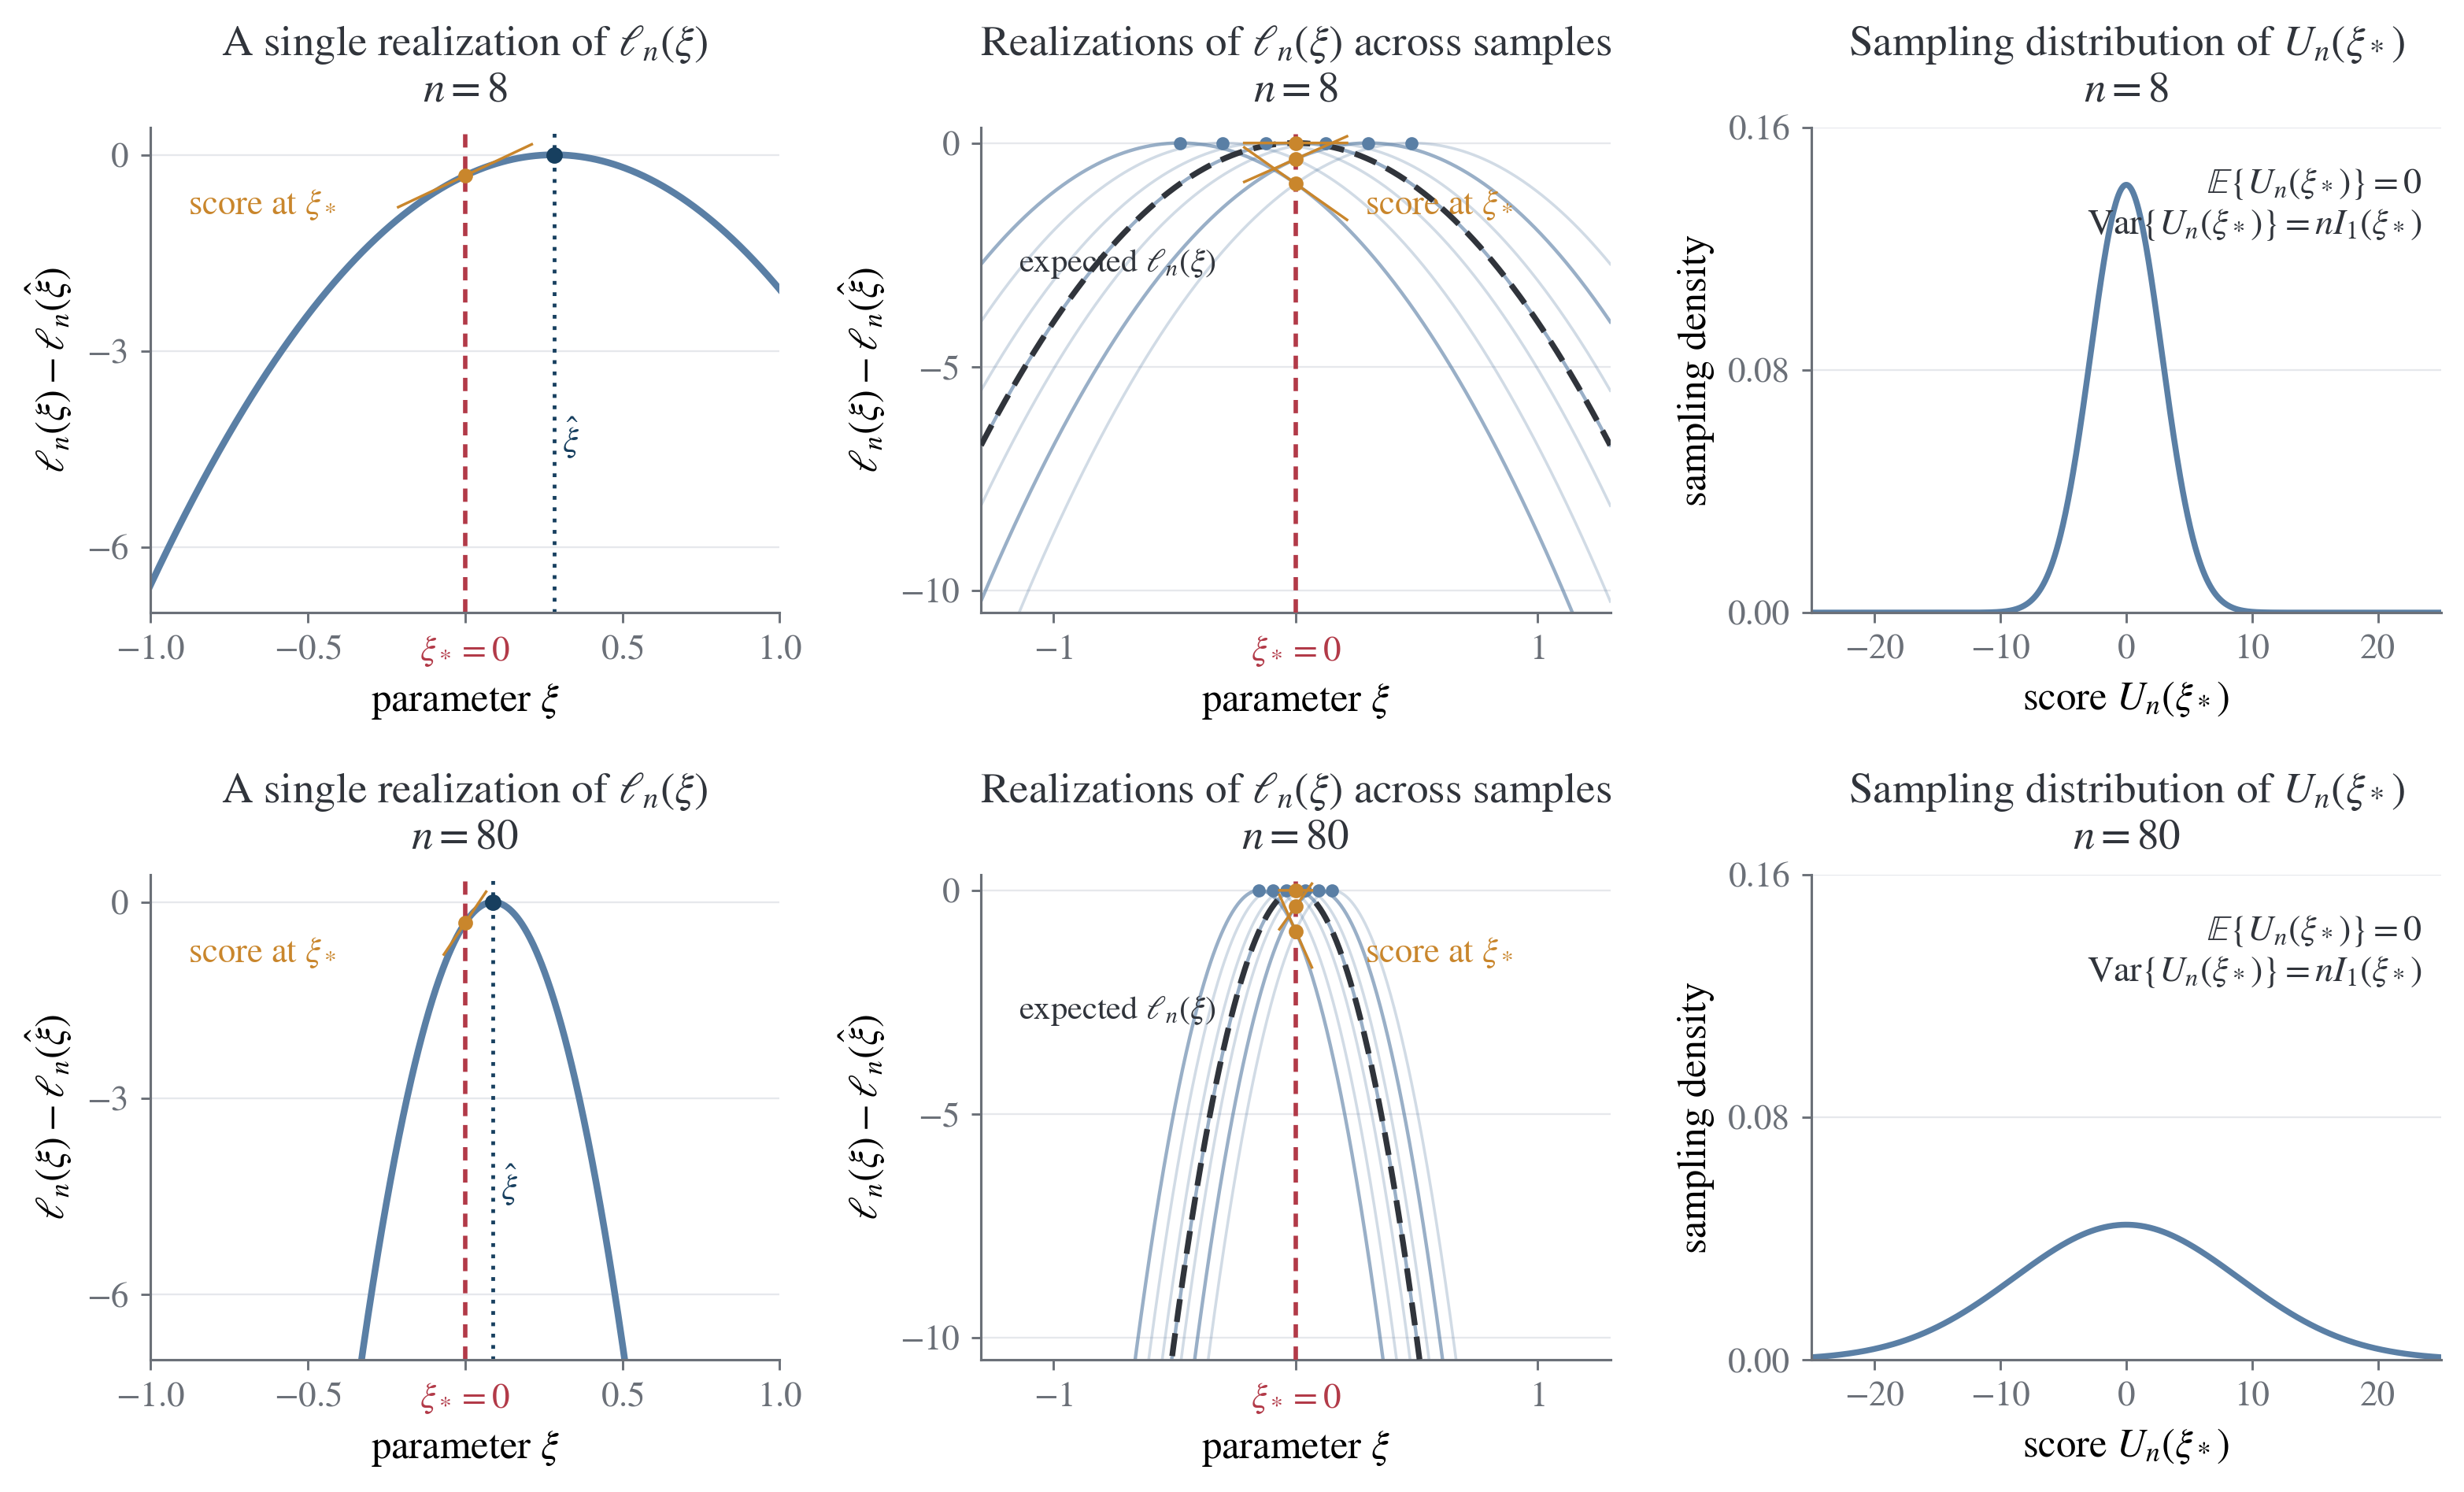
\includegraphics[width=\textwidth]{figures/mle-score-sampling-uncertainty.png}
    \caption{
    \textbf{Score, likelihood curvature, and Fisher information under repeated sampling for a single-parameter model.}\\
    (1) For a regular interior maximum, the MLE $\hat{\xi}$ is obtained by setting the score $U_n(\xi):=\ell_n'(\xi)$ to zero.
    The left column shows one realization of the log-likelihood, while the middle column shows repeated realizations from independent samples of size $n$. The yellow tangent lines and points represent the scores $U_n(\xi_*)$, i.e., the slopes of the realized log-likelihoods at the true parameter $\xi_*$, which fluctuate from sample to sample.\\
    (2) Comparing the top and bottom rows, increasing $n$ makes the log-likelihood more sharply curved downward, so the observed negative curvature $-\ell_n''(\hat{\xi})$ becomes larger in magnitude. At the same time, the total score $U_n(\xi_*)$, being the sum of $n$ individual scores, exhibits greater variability across repeated samples (right column). This larger score variance reflects \emph{more} Fisher information (rather than greater uncertainty about $\xi$) and yields a more concentrated MLE, since the steeper curvature converts a given score perturbation into a smaller displacement of $\hat{\xi}$.\\
    (3) The Bartlett identities formalize this relationship. First, $\E_{\xi_*}[U_n(\xi_*)]=0$, so the score at true $\xi_*$ has mean zero. Moreover, 
    $\E_{\xi_*}[-\ell_n''(\xi_*)]
    =\Var_{\xi_*}[U_n(\xi_*)]
    =\E_{\xi_*}[U_n(\xi_*)^2]
    \stackrel{\mathrm{def}}{=}I_n(\xi_*)$, 
    that is, the expected negative log-likelihood curvature and the score variance are equivalent measures of Fisher information: more observations imply larger curvature, greater score variance, and a more concentrated MLE (i.e., a smaller asymptotic variance). The precise relationships are developed in the following subsections.
    }
    \label{fig:mle-score-sampling-uncertainty}
\end{figure}


\subsubsection{Maximum likelihood estimator} 
The MLE of $\xi$ is $\hat\xi = \argmax_{\xi \in \Xi} \ell_n(\xi)$. 
If $\hat\xi$ is an interior maximizer and $\ell_n$ is twice differentiable, then $\hat\xi$ satisfies
\[
    \ell_n'(\hat{\xi})=0,
    \qquad
    \ell_n''(\hat{\xi})\preceq 0.
\]
If $\ell_n''(\hat{\xi})\prec 0$, then $\hat{\xi}$ is a strict local maximizer. If $\ell_n$ is strictly concave on a convex parameter space (e.g., for regular exponential family distributions), it is the unique global maximizer.

\textbf{Newton-Raphson algorithm:} 
We seek a root of the score equation $\ell_n'(\xi)=0$.
Although this equation typically does not admit a closed-form solution, the MLE $\hat{\xi}$ can be computed numerically using the Newton-Raphson iteration
\footnote{This iteration is obtained by taking the first-order Taylor expansion of the score function $\ell_n'(\xi)$ about $\xi^t$, $\ell_n'(\xi^{t+1}) \approx \ell_n'(\xi^t) + \ell_n''(\xi^t)(\xi^{t+1}-\xi^t)$, and setting the approximation equal to zero to approximate a root of the score equation $\ell_n'(\xi)=0$.}
\begin{mybox}
\begin{equation}\label{eq:newton-raphson}
    \xi^{t+1} = \xi^t - \{\ell_n''(\xi^t)\}^{-1}\ \ell_n'(\xi^t).
\end{equation}
\end{mybox}

The Fisher-scoring method replaces the observed information $-\ell_n''(\xi^t)$ with the Fisher information $I_n(\xi^t)$, which can improve numerical stability, yielding the iteration $\xi^{t+1} = \xi^t + \{I_n(\xi^t)\}^{-1}\ \ell_n'(\xi^t)$.

\subsubsection{Asymptotics of the scores.}
We now present some asymptotic properties of the score and the MLE.

Suppose that $U_1,\ldots,U_n\stackrel{\mathrm{iid}}{\sim}p(u;\xi_*)$, where $\xi_*$ denotes the true value of $\xi$.

In this setting, the log-likelihood can be decomposed as $\ell_n(\xi) = \sum_{i=1}^n \log p(U_i;\xi)$ by independence, and $\E\left[\ell_n(\xi)\right]=n\E\left[\ell_1(\xi)\right]$ since the $U_i$'s are identically distributed.

Assume that the score $\ell_1'(\xi_*)$ has a finite, non-singular single-observation Fisher information matrix (FIM)
\footnote{The FIM is defined as the covariance matrix of the score. Under the usual regularity conditions, the score has mean zero, so the FIM is also its second moment.}:
\begin{mybox}
\begin{equation}\label{eq:singe-FIM}
    I_1(\xi_*)
    =
    \E\left[
        [\ell_1'(\xi_*)][\ell_1'(\xi_*)]^\top
    \right]
    =
    -\E\left[\ell_1''(\xi_*)\right],
\end{equation}
\end{mybox}
where $\ell_1(\xi)=\log p(U_1;\xi)$. The second equality is the Fisher information identity and requires additional regularity conditions and the existence of the expected Hessian.

Then, by the \textbf{LLN}, the observed information per observation satisfies
\[
    -n^{-1}\ell_n''(\xi_*)
    % = -n^{-1}\sum_{i=1}^n \ell_i''(\xi_*)
    \stackrel{a.s.}{\to}
    I_1(\xi_*).
\]
By the \textbf{CLT},
\begin{mybox}
\begin{equation}\label{eq:CLT_scores}
    n^{-1/2}\ell_n'(\xi_*)
    % = n^{-1/2}\sum_{i=1}^n \ell_i'(\xi_*)
    \stackrel{d}{\to}
    N\left(0,I_1(\xi_*)\right).
\end{equation}
\end{mybox}
In practice, the true parameter $\xi_*$ is unknown and is replaced by the MLE $\hat\xi$. Under regularity conditions, since $\hat\xi \stackrel{\mathrm{a.s.}}{\to} \xi_*$, the observed Fisher information per observation $-n^{-1}\ell_n''(\hat\xi)$ is a consistent estimator of $I_1(\xi_*)$.

\textbf{Remark:} When $U_1,\ldots,U_n$ are independent with common true parameter $\xi_*$ but not necessarily identically distributed, let $I_n(\xi_*)=\sum_{i=1}^n I_{U_i}(\xi_*)$ denote the FIM based on $n$ observations. Similar results hold under regularity conditions if
\[
    n^{-1} I_n(\xi_*) = n^{-1} \sum_{i=1}^n I_{U_i}(\xi_*)
    \to I(\xi_*).
\]
In this case,
\[
    n^{-1/2}\ell_n'(\xi_*)
    \stackrel{d}{\to}
    N\left(0,I(\xi_*)\right),
    \qquad
    -n^{-1}\ell_n''(\xi_*)
    \stackrel{p}{\to}
    I(\xi_*).
\]


\subsubsection{Asymptotics of the MLE.}
The asymptotics of the score allow us to derive the asymptotics of the MLE $\hat\xi$ through a Taylor expansion of the score equation. Let $\Delta\xi=\hat\xi-\xi_*$. For an interior MLE and a sufficiently smooth log-likelihood,
\[
    0
    =\ell_n'(\hat\xi)
    =\ell_n'(\xi_*)
    +\ell_n''(\xi_*)\Delta\xi
    +\frac{1}{2}\Delta\xi^\top
      \left[\ell_n'''(\tilde\xi)\Delta\xi\right],
\]
for some $\tilde\xi$ between $\xi_*$ and $\hat\xi$. 
\footnote{The displayed second-order expansion is intended only as an illustration and is not technically correct as written in the multivariate case: $\ell_n'''$ is a third-order tensor, and a single intermediate point $\tilde\xi$ need not work for every score component. A dimensionally correct exact expansion is
\[
    0
    =\ell_n'(\hat\xi)
    =\ell_n'(\xi_*)
    +\left\{\int_0^1\ell_n''(\xi_*+t\Delta\xi)\,dt\right\}\Delta\xi.
\]
Further details involving this expansion are beyond the scope of these notes and are omitted.
}
Many asymptotic results in this course are established similarly by first applying a Taylor expansion and then invoking CLT and LLN. Also see Section \ref{sec:misc-asymptotics} for small $o$ and big $O$ notations.

Suppose that $U_1,\ldots,U_n$ are i.i.d. and that the likelihood is correctly specified. We have the following results.

\textbf{Consistency:} Under suitable regularity conditions, $\hat{\xi} \stackrel{a.s.}{\to} \xi_*$.

\textbf{Asymptotic normality:} Under additional suitable regularity conditions\footnote{Asymptotic normality usually requires more regularity conditions than consistency.},
\begin{mybox}
\begin{equation}\label{eq:mle-clt}
    \sqrt{n}(\hat{\xi}-\xi_*)
    \stackrel{d}{\rightarrow}
    N\left(0,I_{1}(\xi_*)^{-1}\right).
\end{equation}
\end{mybox}

\textbf{Remark:} When $U_1,\ldots,U_n$ are independent with common true parameter $\xi_*$ but not necessarily identically distributed, suppose that
\[
    n^{-1}I_n(\xi_*)\to I(\xi_*),
\]
where $I(\xi_*)$ is the limiting average FIM per observation, assumed to be positive definite. Under suitable regularity conditions, $\hat\xi \stackrel{a.s.}{\to} \xi_*$, and the analogous asymptotic normality result is
\[
    \sqrt{n}(\hat{\xi}-\xi_*)
    \stackrel{d}{\rightarrow}
    N\left(0,I(\xi_*)^{-1}\right).
\]


\subsubsection{More results that justify MLE.}
Consider the log-likelihood-ratio criterion
\footnote{$-M(\xi) = D_\mathrm{KL}(p_{\xi_*} || p_\xi)$ is the Kullback-Leibler divergence of $p_{\xi_*}$ from $p_\xi$.}:
\begin{align*}
    M(\xi) &= \E\Big[\log \frac{p(U_1; \xi)}{p(U_1; \xi_*)}\Big] \qquad \text{(population criterion)}\\
    M_n(\xi) &= n^{-1} \sum_{i=1}^n \log \frac{p(U_i; \xi)}{p(U_i; \xi_*)} \qquad \text{(sample criterion)}
\end{align*}

\paragraph{Result 0.} The MLE $\hat\xi$ maximizes $M_n(\xi)$.

\paragraph{Result 1 (Lemma 2.1): The population criterion $M(\xi)$ is uniquely maximized at $\xi_*$.}
If the model $p(U;\xi)$ is identifiable, then $M(\xi)$ attains its maximum uniquely at $\xi_*$.
\footnote{The implication is that, if $\xi_*$ is an interior point and $M$ is differentiable at $\xi_*$, then $\partial_\xi M(\xi_*)=0$. In practice, we locate interior MLE candidates by solving $\partial_\xi M_n(\xi)=0$, equivalently $\ell_n'(\xi)=0$, and then determine which candidate maximizes $M_n(\xi)$.}

\paragraph{Result 2 (Theorem 2.4): MLE is consistent.} If $M_n$ converges uniformly in probability to $M$ and $M$ has a well-separated peak at $\xi_*$ (that is, values of $M$ away from $\xi_*$ remain noticeably below its maximum $M(\xi_*)$), then $\hat\xi \stackrel{p}{\to} \xi_*$.

\paragraph{Result 3 (Theorem 2.5): MLE is asymptotically normal.} This is stated in \eqref{eq:mle-clt}.

\subsection{Continuous mapping theorem and Delta method}\label{sec:prelim-glm-cmt-delta}
As a preparation for the classical hypothesis testing procedures, we introduce some useful tools for deriving the asymptotic distribution of a smooth function $h(\hat{\xi})$ from that of $\hat\xi$.

Suppose that $h(\xi_*)$ is the parameter of interest. A natural estimator of $h(\xi_*)$ is the plug-in estimator $h(\hat{\xi})$.

\textbf{Theorem 2.6}
\begin{enumerate}
  \item (CMT) If $h$ is continuous at $\xi_*$ and $\hat{\xi} \stackrel{p}{\to} \xi_*$, then $h(\hat{\xi}) \stackrel{p}{\to} h(\xi_*)$.
  %
  \item (First-order Delta method) If $h$ is differentiable at $\xi_*$ and $\sqrt{n}(\hat{\xi} - \xi_*) \stackrel{d}{\to} N(0, I_1(\xi_*)^{-1})$, then 
    \[
    \sqrt{n}(h(\hat{\xi}) - h(\xi_*)) \stackrel{d}{\to} N(0, h'(\xi_*) I_1(\xi_*)^{-1} h'(\xi_*)^\top).
    \]
    In practice, $h'(\xi_*)$ is replaced by $h'(\hat\xi)$.
\end{enumerate}



\subsection{Three hypothesis testing procedures}\label{sec:prelim-glm-three-tests}
\subsubsection{Testing general hypotheses}
We consider testing linear or nonlinear hypotheses of the form
\[
    H_0: h(\xi)=b
    \qquad \text{vs.} \qquad
    H_1: h(\xi)\neq b,
\]
where $h(\cdot)$ is an $r \times 1$ vector-valued function of the $q$-dimensional parameter $\xi$, with $r \leq q$, and $b \in \R^r$. 
Here, $\xi$ denotes the unknown true parameter value generating $U_1,\ldots,U_n$.

(In previous sections, the true parameter was denoted by $\xi_*$. For simplicity, we suppress the subscript and write $\xi$ throughout this section.)

We present three classical tests for this problem: \textbf{the Wald test, the score test, and the likelihood ratio test (LRT)}. Under standard regularity conditions, the three tests are asymptotically equivalent to first order, but generally differ in their second-order asymptotic behavior.
We shall see that the Wald test and the score test are derived from the previous asymptotic properties of MLE.

\begin{mybox}
We use $\hat\xi$ to denote the unrestricted MLE, obtained by maximizing the likelihood over the entire parameter space, and $\hat\xi_0$ to denote the restricted MLE under the null hypothesis $H_0: h(\xi)=b$.

\textbf{The Wald test.}
\begin{equation}\label{Wald-test}
    W_n = [h(\hat\xi) - b]^\top \left[h'(\hat\xi)\ I_n^{-1}(\hat\xi)\ h'(\hat\xi)^\top\right]^{-1} [h(\hat\xi) - b],
\end{equation}
where $h'(\xi) = \left[ \frac{\partial h_i(\xi)}{\partial \xi_j} \right]_{ij}$ is the $r\times q$ Jacobian matrix of $h$. Here, $I_n(\hat\xi) = \E[\ell_n'(\hat\xi) \ell_n'(\hat\xi)^\top] = \E[-\ell_n''(\hat\xi)]$ is the FIM evaluated at \emph{unrestricted} MLE $\hat\xi$ and can be replaced by $-\ell_n''(\hat\xi)$ in practice.

\textbf{The score test.}
\begin{equation}\label{Score-test}
    SC_n = \ell_n'(\hat\xi_0)^\top \left[ I_n(\hat\xi_0) \right]^{-1} \ell_n'(\hat\xi_0),
\end{equation}
where $I_n(\hat\xi_0) = \E[\ell_n'(\hat\xi_0) \ell_n'(\hat\xi_0)^\top] = \E[-\ell_n''(\hat\xi_0)]$ is the FIM evaluated at \emph{restricted} MLE $\hat\xi_0$ and can be replaced by $-\ell_n''(\hat\xi_0)$ in practice.

\textbf{The LRT.}
\begin{equation}\label{LR-test}
    LRT_n = 2[\ell_n(\hat\xi) - \ell_n(\hat\xi_0)].
\end{equation}
    
\textbf{All three tests are asymptotically $\chi^2(r)$ under $H_0$.}
\end{mybox}


\textbf{Remark:} 
The Wald test only depends on the unrestricted MLE $\hat{\xi}$.
The score test only depends on the restricted MLE $\hat\xi_0$.
The LRT depends on both.

\textbf{Rationale:}

\begin{itemize}
    \item The Wald test can be motivated informally from the asymptotic behavior of the MLE:
    \begin{align*}
        & \hat\xi-\xi
        \stackrel{d}{\to}
        N_q\big(0,[I_n(\xi)]^{-1}\big)
        &\text{(informal statement)}\\
        \Rightarrow\quad
        & h(\hat\xi)-b
        \stackrel{d}{\to}
        N_r\big(0,h'(\xi)[I_n(\xi)]^{-1}h'(\xi)^\top\big)
        &\text{(Delta method and $h(\xi)=b$ under $H_0$)}\\
        \Rightarrow\quad
        & W_n\stackrel{d}{\to}\chi^2(r)
        \quad\text{under $H_0$}
        &\text{(replace $\xi$ by $\hat\xi$ in the covariance).}
    \end{align*}
    Assuming that $I_n(\xi)$ is nonsingular and $h'(\xi)$ has full row rank $r$, the displayed covariance matrix has rank $r$.

    \item The score test can be motivated from the asymptotic behavior of the score. Informally,
    \footnote{
        \textbf{Caveat:}
        The two displayed normal convergence statements for the Wald and score tests are not mathematically correct and are included only to illustrate the motivation. In the i.i.d. setting, the correct statements normalize the left-hand sides, yielding
        \[
        \sqrt{n}(\hat\xi-\xi) \stackrel{d}{\to} N_q\big(0,I_1(\xi)^{-1}\big), 
        \quad
        n^{-1/2}\ell_n'(\xi) \stackrel{d}{\to} N_q\big(0,I_1(\xi)\big).
        \]
    }
    \[
        \ell_n'(\xi)
        \stackrel{d}{\to}
        N_q\big(0,I_n(\xi)\big)
        \quad\Rightarrow\quad
        \ell_n'(\xi)^\top[I_n(\xi)]^{-1}\ell_n'(\xi)
        \stackrel{d}{\to}\chi^2(q).
    \]
    Under $H_0$, the restricted MLE $\hat\xi_0$ is consistent for the true parameter $\xi$. 
    Since $H_0$ imposes $r$ independent restrictions, the degrees of freedom is $r$ rather than $q$. Thus, evaluating the score at the restricted MLE $\hat\xi_0$ yields
    \[
        SC_n\stackrel{d}{\to}\chi^2(r).
    \]
    \item If you are interested, here are some lemmas that establish the first-order asymptotic equivalence between the three test statistics.\footnote{See their proofs on p. 93 of the \textit{Testing Statistical Hypotheses} chapter in BIOS761 Slides.} The rationale is also illustrated in Figures \ref{fig:mle-score-sampling-uncertainty} and \ref{fig:three-classical-tests}. For a simple null $H_0:\theta=\theta_0$, under suitable regularity conditions,
    \begin{align*}
      \text{Lemma 1.}\quad
      & \sqrt{n} (\hat\theta-\theta) = I_1(\theta)^{-1} \big[n^{-1/2} \ell_n'(\theta)\big] +o_p(1).
      &\qquad\text{(connects Wald and Score)}\\
      \text{Lemma 2.}\quad
      & 2\{\ell_n(\hat\theta)-\ell_n(\theta)\} = n(\hat\theta-\theta)^\top I_1(\theta) (\hat\theta-\theta) +o_p(1).
      &\qquad\text{(connects LRT and Wald)}\\
      \text{Lemmas 1 and 2 imply:}\quad
      & 2\{\ell_n(\hat\theta)-\ell_n(\theta)\} = n^{-1} \ell_n'(\theta)^\top I_1(\theta)^{-1}\ell_n'(\theta) +o_p(1).
      &\qquad\text{(connects LRT and Score)}\\
    \end{align*}
\end{itemize}

\begin{figure}[!h]
    \centering
    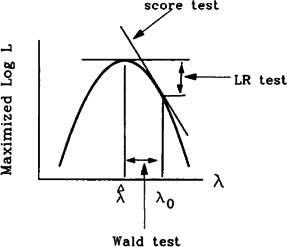
\includegraphics[width=0.4\textwidth]{figures/three-classical-test.jpg}
    \caption{Heuristic illustration of the Wald test, the score test, and the likelihood ratio test for testing the one-dimensional hypothesis $H_0:\lambda=\lambda_0$.
    \href{https://methods.sagepub.com/book/mono/regression-diagnostics/chpt/maximumlikelihood-methods-score-tests-constructed}{Source}.}
    \label{fig:three-classical-tests}
\end{figure}

\subsubsection{Testing linear hypotheses}
(Results copied from the lecture slides for completeness.)

In particular, consider testing a linear hypothesis of the form
\[
    H_0: R\xi=b
    \qquad \text{vs.} \qquad
    H_1: R\xi\neq b,
\]
where $R \in \R^{r \times q}$ has full row rank, with $r \leq q$.

Without loss of generality, after a nonsingular linear reparameterization, we may assume that $R = (I_r,0)$ and partition $\xi = \left(\xi(1)^\top,\xi(2)^\top\right)^\top$, where $\xi(1)$ and $\xi(2)$ are $r \times 1$ and $(q-r) \times 1$ subvectors of $\xi$, respectively. Then $R\xi=\xi(1)$, and the linear hypothesis becomes
%
\begin{equation*}
  H_0: \xi(1) = b
  \qquad \text{vs.} \qquad
  H_1: \xi(1) \ne b
\end{equation*}
%

Write the unrestricted MLE of $\xi$ as $\hat{\xi} = (\hat{\xi}(1)^\top,\hat{\xi}(2)^\top)^\top$. For each fixed $\xi(1)$, let $\hat{\xi}(2)[\xi(1)]$ denote the value of $\xi(2)$ that maximizes the log likelihood. Thus, under $H_0$, the restricted MLE is $\hat{\xi}_0 = (b^\top,\hat{\xi}_0(2)^\top)^\top$, where $\hat{\xi}_0(2)=\hat{\xi}(2)[b]$.

According to the partition $\xi = \left(\xi(1)^\top,\xi(2)^\top\right)^\top$, define the partitioned score, Hessian, and inverse Hessian by
\begin{align*}
  \ell_n'(\xi)
  &= \begin{pmatrix}
    \dot{L}_1(\xi) \\
    \dot{L}_2(\xi)
  \end{pmatrix}, \\
  \ell_n''(\xi)
  &= \ddot{L}(\xi)
  = \begin{pmatrix}
    L_{11}(\xi) & L_{12}(\xi) \\
    L_{21}(\xi) & L_{22}(\xi)
  \end{pmatrix}, \\
  [\ell_n''(\xi)]^{-1}
  &= \ddot{L}(\xi)^{-1}
  = \begin{pmatrix}
    L^{11}(\xi) & L^{12}(\xi) \\
    L^{21}(\xi) & L^{22}(\xi)
  \end{pmatrix}.
\end{align*}
Here, $\dot{L}_1(\xi) \in \R^r$ and $\dot{L}_2(\xi) \in \R^{q-r}$, while $L_{11}(\xi), L^{11}(\xi) \in \R^{r \times r}$. The superscripts index blocks of the inverse Hessian; in general, $L^{11}(\xi) \ne L_{11}(\xi)^{-1}$.

The Wald test statistic is
\begin{align*}
  W_n &= (\hat{\xi}(1) - b)^\top [\Cov(\hat{\xi}(1))]^{-1} (\hat{\xi}(1) - b) \\
  %
    &= (\hat{\xi}(1) - b)^\top [R I_n(\hat{\xi})^{-1} R^\top]^{-1} (\hat{\xi}(1) - b),
\end{align*}
where $I_n(\xi)=\E[-\ell_n''(\xi)]$ is the FIM, evaluated at the unrestricted MLE $\hat{\xi}$.

Equivalently, using the observed information $-\ell_n''(\hat{\xi})$, we estimate $\Cov(\hat{\xi}(1))$ by $-L^{11}(\hat{\xi})$.

The score test statistic is
\begin{equation*}
  \text{SC}_n = -\dot{L}_1(\hat{\xi}_0)^\top L^{11}(\hat{\xi}_0) \dot{L}_1(\hat{\xi}_0).
\end{equation*}
Here, both $\dot{L}_1(\hat{\xi}_0)$ and $L^{11}(\hat{\xi}_0)$ are evaluated at the restricted MLE. Because $\hat{\xi}_0(2)$ maximizes the log likelihood under $H_0$, $\dot{L}_2(\hat{\xi}_0)=0$, whereas $\dot{L}_1(\hat{\xi}_0)$ need not be zero.


\subsection{Exponential family}\label{sec:prelim-glm-exp-family}
\subsubsection{Definition of univariate exponential family}
\textbf{Definition:} (Univariate exponential Family) \\
If the density of a random variable $Y$ 
% with respect to a $\sigma$-finite measure $\Lambda(y)$ 
has the form
\begin{mybox}
\begin{equation}\label{eq:prelim-glm-exp-family-form}
  p(y | \xi) = \exp 
  \left\{
    \phi[y\theta - b(\theta) - c(y)] - \frac{1}{2} s(y, \phi)
  \right\}
\end{equation}
\end{mybox}
where $\xi = (\theta, \phi)$, $c(\cdot), b(\cdot)$ and $s(\cdot,\cdot)$ are some known functions, then $Y$ or its distribution belongs to a \emph{(univariate) exponential family}, denoted by $Y \sim D(\theta, \phi)$. In addition, $\theta$ is the \emph{natural parameter} of the exponential family and $\phi$ is the \emph{precision parameter}.
\footnote{The lecture slides refer to $\phi$ as the dispersion parameter. Under the conventional parameterization of exponential families, however, the dispersion parameter is typically $1/\phi$. We therefore refer to $\phi$ as the precision parameter here.}

\textbf{Note:} The support $\mathcal{Y}=\{y:p(y |\xi)>0\}$ must not depend on the unknown parameter $\xi$.

\subsubsection{Properties of univariate exponential family}
\textbf{MGF and CGF:} 
\[
M_Y(t) = \exp\Big\{\phi\big[b(\theta + t/\phi) - b(\theta)\big]\Big\}
\qquad
K_Y(t) = \log M_Y(t) = \phi[b(\theta + t/\phi) - b(\theta)]
\]

\textbf{Central moments:}
\begin{mybox}
\begin{equation}\label{eq:prelim-glm-exp-family-moments}
    \E[Y] = b'(\theta), 
    \qquad
    \Var(Y) = \phi^{-1} b''(\theta),
    \qquad
    \E[(Y - \E[Y])^3] = \phi^{-2} b'''(\theta).
\end{equation}
\end{mybox}
Here, primes denote derivatives with respect to the natural parameter $\theta$.

\textbf{Reparametrization:} Under proper conditions, $\mu := \E[Y] = b'(\theta)$ is a one-to-one function of the natural parameter $\theta$ (i.e., $b'$ is bijective), which allows us to reparametrize the sampling model with $\mu$ (see Slides p. 498). We then have
\[
\partial_\theta \mu = b''(\theta),\qquad \partial_\mu\theta = \{b''(\theta)\}^{-1}.
\]

\textbf{MLE properties.}
Let $Y_1,\ldots,Y_n\overset{\mathrm{iid}}{\sim}D(\theta,\phi)$, where $\xi=(\theta,\phi)$, $\phi>0$, and the support does not depend on $\xi$. The log-likelihood is given by
\begin{mybox}
\begin{equation}\label{eq:prelim-glm-exp-family-loglike}
    \ell_n(\phi,\theta)
    =
    \phi\left[
        \big(\sum_{i=1}^n y_i\big)\theta
        -nb(\theta)
        -\sum_{i=1}^n c(y_i)
    \right]
    -\frac{1}{2}\sum_{i=1}^n s(y_i,\phi).
\end{equation}
\end{mybox}

\textbf{MLE of $\theta$:} The score and Hessian with respect to $\theta$ are
\[
    \partial_\theta\ell_n(\phi,\theta)
    =n\phi\{\bar y-b'(\theta)\},
    \qquad
    \partial_\theta^2\ell_n(\phi,\theta)
    =-n\phi b''(\theta)<0,
\]
where $b''(\theta)=\phi\Var(Y)>0$ for a nondegenerate exponential family (namely, $\Var(Y) > 0$). 
Therefore, for every fixed $\phi>0$, the log-likelihood is strictly concave in $\theta$ and any interior MLE $\hat\theta$ is unique.
\footnote{A finite interior MLE exists when $\bar y\in\operatorname{int}\{b'(\Theta)\}$. If $\bar y$ lies on the boundary, regular score-equation and asymptotic-normality theory cannot be applied without modification. For example, the score need not be zero at a boundary maximizer.}

Any interior MLE satisfies
\[
    \partial_\theta\ell_n(\hat\phi,\hat\theta)=0
    \quad\Leftrightarrow\quad
    b'(\hat\theta)=\bar y.
\]
Because $\mu=b'(\theta)$, we have $\hat\mu=b'(\hat\theta)=\bar y$. 
In other words, for IID samples from a one-parameter exponential family distribution, whenever a finite interior MLE exists, the MLE of the mean parameter is always the sample mean.

Moreover, if the inverse of $b'$ is available in closed form, then the MLE of $\theta$ is
\[
    \hat\theta=(b')^{-1}(\hat\mu)=(b')^{-1}(\bar y).
\]
If the inverse is not available in closed form, Newton-Raphson can be applied to the score equation $\bar y-b'(\theta)=0$, giving
\[
    \theta^{t+1}
    =
    \theta^t
    +\{b''(\theta^t)\}^{-1}
    \{\bar y-b'(\theta^t)\}.
\]

\textbf{MLE of $\phi$:} Differentiating the log-likelihood with respect to $\phi$ gives
\[
    \partial_\phi\ell_n(\phi,\theta)
    =
    \big(\sum_{i=1}^n y_i \big) \theta
    -nb(\theta)
    -\sum_{i=1}^n c(y_i)
    -\frac{1}{2}\sum_{i=1}^n\partial_\phi s(y_i,\phi).
\]
Therefore, the joint interior MLE $(\hat\theta,\hat\phi)$ satisfies
\[
    \frac{1}{2}\sum_{i=1}^n\partial_\phi s(y_i,\hat\phi)
    =
    \big(\sum_{i=1}^n y_i \big) \hat\theta
    -nb(\hat\theta)
    -\sum_{i=1}^n c(y_i).
\]

\subsubsection{Multivariate exponential family}
In general, exponential families can be defined for multi-dimensional $\theta$ and $y$. A \emph{multivariate exponential family (MEF)} is defined as
\begin{equation*}
  p(y | \xi) = \exp 
  \left\{
    Q(y)^\top T(\theta) - b(\theta) - c(y)
  \right\}
\end{equation*}
where $\xi = \theta$, $T(\theta) = (t_1(\theta), \ldots t_k(\theta))^\top$, and 
$Q(y) = (q_1(y), \ldots, q_k(y))^\top$. 
Let $\mathcal{H}=\{T(\theta):\theta\in\Theta\}$ denote the natural parameter space. The exponential family is \emph{full} if $\mathcal{H}$ contains a nonempty open subset of $\R^k$.
\footnote{The lecture notes instead describe the family as having \emph{full rank} when the components of $T(\theta)$ and $Q(y)$ are linearly independent. This is a simplified, nonstandard characterization: fullness asks whether the natural parameter space $\mathcal{H}$ is full-dimensional in $\R^k$, whereas minimality asks whether $Q(y)$ is free of redundant sufficient statistics.}


\section{Generalized linear model}\label{sec:glm}
The main results are covered in Slides pp. 600-650.

\subsection{Formulation}\label{sec:glm-formulation}
\textbf{Sampling model:} For $i=1,\ldots,n$, let $x_i\in\R^p$ be the covariate vector. Conditional on $x_1,\ldots,x_n$, the responses $y_1,\ldots,y_n$ are independent, with
\[
y_i | x_i\sim D(\theta_i,\phi/\omega_i),
\]
where $D(\theta_i,\phi/\omega_i)$ denotes a distribution in the exponential family, $\theta_i$ is its natural parameter, and $\phi/\omega_i$ is its observation-specific precision parameter; $\phi>0$ is a common precision scale that may be known or unknown, and $\omega_i>0$ is a given relative-variance factor.

\textbf{Model:} The conditional mean $\mu_i=\E[y_i | x_i]$ is related to the linear predictor $\eta_i$ through a \emph{link function} $g$ such that
\[
g(\mu_i) = \eta_i \stackrel{\mathrm{def}}{=}x_i^\top\beta,
\]
where $\beta=(\beta_1,\ldots,\beta_p)^\top$ is defined in a subset $\mathcal{B}\subseteq\R^p$ with $p < n$, and $g$ is a known monotone link function.

Recall that $\mu_i=b'(\theta_i)$ for the exponential family. Assuming $b'$ is invertible, the relationships among the natural parameter, conditional mean, and linear predictor are summarized by
\begin{mybox}
\begin{equation}\label{eq:GLM-relationship}
    \theta_i
    \xrightleftharpoons[(b')^{-1}(\cdot)]{b'(\cdot)}
    \mu_i=\E[y_i | x_i]
    \xrightleftharpoons[g^{-1}(\cdot)]{g(\cdot)}
    \eta_i=x_i^\top\beta.
\end{equation}
\end{mybox}
Thus,
\begin{align*}
  \mu_i &= g^{-1}(x_i^\top\beta), \\
  \theta_i &= (b')^{-1}\circ g^{-1}(x_i^\top\beta)
  =k(x_i^\top\beta),
\end{align*}
where $k=(b')^{-1}\circ g^{-1}$. The link is \emph{canonical} when $g=(b')^{-1}$; then $\theta_i=\eta_i=x_i^\top\beta$ and $k$ is the identity function. In other words, under the canonical link, the natural parameters are directly modeled by the linear predictors.


\subsection{Estimation methods}\label{sec:glm-estimation}
For the remainder of this section, suppose $\omega_i=1$ and $\phi$ is unknown, and let $\xi=(\beta^\top,\phi)^\top$. If $\phi$ is known, the formulas for $\beta$ remain unchanged, while the estimation and information components involving $\phi$ are omitted. 

The log-likelihood is
\[
  \ell_n(\xi)
  =\phi\sum_{i=1}^n
  \Big[
    \underbrace{y_i k(x_i^\top\beta)
    -b\{k(x_i^\top\beta)\}}_{= y_i \theta_i - b(\theta_i)}
    -c(y_i)
  \Big]
  -\frac{1}{2}\sum_{i=1}^n s(y_i,\phi).
\]
The joint MLE $\hat\xi=(\hat\beta^\top,\hat\phi)^\top$ can be obtained in two steps:
\begin{enumerate}
  \item Compute the MLE of $\beta$:
  \[
    \hat\beta
    =\argmax_{\beta\in\mathcal{B}}
    \sum_{i=1}^n
    \left[
      y_i k(x_i^\top\beta)
      -b\{k(x_i^\top\beta)\}
      -c(y_i)
    \right].
  \]
  \item Given $\hat\beta$, compute the MLE of $\phi$:
  \[
    \hat\phi
    =\argmax_{\phi>0}
    \left\{
      \phi\sum_{i=1}^n
      \left[
        y_i k(x_i^\top\hat\beta)
        -b\{k(x_i^\top\hat\beta)\}
        -c(y_i)
      \right]
      -\frac{1}{2}\sum_{i=1}^n s(y_i,\phi)
    \right\}.
  \]
\end{enumerate}

\subsubsection{Estimating $\beta$}
For notational simplicity, we write $\ell_n(\beta)$ for the log-likelihood as a function of $\beta$ with $\phi$ fixed and suppress the dependence on $\beta$ from the matrix quantities defined below. All derivatives are taken with respect to $\beta$.

The score and Hessian with respect to $\beta$ are
\begin{align*}
  \ell_n'(\beta)
  &=\phi\sum_{i=1}^n
  \left[y_i-b'\{k(x_i^\top\beta)\}\right]
  k'(x_i^\top\beta)x_i, \\
  \ell_n''(\beta)
  &=-\phi\sum_{i=1}^n
  b''\{k(x_i^\top\beta)\}
  \{k'(x_i^\top\beta)\}^2x_ix_i^\top \\
  &\quad+\phi\sum_{i=1}^n
  \left[y_i-b'\{k(x_i^\top\beta)\}\right]
  k''(x_i^\top\beta)x_ix_i^\top.
\end{align*}
Here, note that $b'\{k(x_i^\top\beta)\} = b'(\theta_i) = \mu_i$.


To write these quantities in matrix form, define
\begin{align*}
  y &:= (y_1,\ldots,y_n)^\top, \\
  \theta &:= (\theta_1(\beta),\ldots,\theta_n(\beta))^\top, \\
  \mu &:= (\mu_1(\beta),\ldots,\mu_n(\beta))^\top, \\
  e &:= y - \mu \in \R^n, \\
  D_\beta\theta
  &:=\left[\frac{\partial\theta_i(\beta)}{\partial\beta_j}\right]_{
  ij}
  \in\R^{n\times p}, \\
  D_\beta\mu
  &:=\left[\frac{\partial\mu_i(\beta)}{\partial\beta_j}\right]_{
  ij}
  \in\R^{n\times p}, \\
  V &:= \diag\{v_1(\beta),\ldots,v_n(\beta)\},
\end{align*}
where
\[
  v_i:=b''\{\theta_i(\beta)\}
  =b''\{(b')^{-1}(\mu_i)\}
  =b''\{k(x_i^\top\beta)\}
\]
and $\Var(y_i | x_i)=\phi^{-1}v_i$. 
Note that, since $\mu_i=b'(\theta_i)$, we have $D_\theta\mu=V\in\R^{n\times n}$, and the two Jacobians satisfy
\[
  D_\beta\mu=V D_\beta\theta,
\]
which may be helpful when deriving the MLE quantities (e.g., $\ell_n'(\beta)$ below).

\textbf{Lemma 3.1} (GLM score and Fisher information in matrix form) \\
The score function and Fisher information for $\beta$ are
\begin{align*}
  \ell_n'(\beta)
  &=\phi(D_\beta\theta)^\top e
  =\phi(D_\beta\mu)^\top V^{-1}e, \\
  I_n(\beta)
  &:=\E[\ell_n'(\beta)\ell_n'(\beta)^\top]
  =\phi(D_\beta\theta)^\top V D_\beta\theta \\
  &=\E[-\ell_n''(\beta)]
  =\phi(D_\beta\mu)^\top V^{-1} D_\beta\mu.
\end{align*}
\footnote{
    Here, the only random quantity is $e$. Note that $\E(e)=0_n$ and $\E(ee^\top)=\Cov(e)=\Cov(y-\mu)=\Cov(y)=\phi^{-1}V$.
}
\footnote{
    Note that $I_n(\beta) =\sum_{i=1}^n \frac{1}{\Var(y_i | x_i)} \left[\frac{\partial\mu_i}{\partial\beta}\right] \left[\frac{\partial\mu_i}{\partial\beta}\right]^\top$.
    Here, $1/\Var(y_i | x_i)$ is the conditional precision of observation $i$, while $\partial\mu_i/\partial\beta$ is the sensitivity of its conditional mean to $\beta$. Thus, the Fisher information is a precision-weighted sum of the outer products of the mean sensitivity vectors.
}

\textbf{Newton-Raphson and Fisher scoring.}
Newton-Raphson uses the observed information $-\ell_n''(\beta)$, whereas Fisher scoring replaces it with its conditional expectation $I_n(\beta)$. This yields
\begin{align*}
  \beta^{(m+1)}
  &=\beta^{(m)}
  +I_n(\beta^{(m)})^{-1}\ell_n'(\beta^{(m)}) \\
  &=\beta^{(m)}
  +\left.
  \left[(D_\beta\mu)^\top V^{-1} D_\beta\mu\right]^{-1}
  (D_\beta\mu)^\top V^{-1}e
  \right|_{\beta=\beta^{(m)}},
\end{align*}
where $m=0,1,2,\ldots$ indexes the iterations.

\subsubsection{Estimating $\phi$ (less essential)}
Fix the estimate $\hat\beta$ from the first step. 
For notational simplicity, we write $\ell_n(\phi):=\ell_n(\hat\beta,\phi)$ and suppress the dependence on $\hat\beta$. Define
\[
  d_i
  :=y_i k(x_i^\top\hat\beta)
  -b\{k(x_i^\top\hat\beta)\}
  -c(y_i).
\]
The score, observed information, and Fisher information for $\phi$ are
\[
  \ell_n'(\phi)
  =\sum_{i=1}^n d_i
  -\frac{1}{2}\sum_{i=1}^n s'(y_i,\phi), \quad
  -\ell_n''(\phi)
  =\frac{1}{2}\sum_{i=1}^n s''(y_i,\phi), \quad
  I_n(\phi)
  =\frac{1}{2}\sum_{i=1}^n
  \E[s''(y_i,\phi)].
\]
Here, the primes on $s(y,\phi)$ denote derivatives with respect to $\phi$. The Newton-Raphson update is
\[
  \phi^{(m+1)}
  =\phi^{(m)}
  +\left\{\frac{1}{2}\sum_{i=1}^n
  s''(y_i,\phi^{(m)})\right\}^{-1}
  \left\{\sum_{i=1}^n d_i
  -\frac{1}{2}\sum_{i=1}^n s'(y_i,\phi^{(m)})\right\},
  \qquad m=0,1,2,\ldots.
\]


\subsection{GLM likelihood theory}\label{sec:glm-likelihood-theory}
\subsubsection{MLE properties}
Let $\xi_*=(\beta_*^\top,\phi_*)^\top$ denote the true parameter value.

\textbf{Consistency.} Under suitable regularity conditions, $\hat\xi \stackrel{p}{\to} \xi_*$.

\textbf{Asymptotic normality.} Under suitable regularity conditions,
\[
  \sqrt{n}(\hat\xi-\xi_*)
  \xrightarrow{d}
  N_{p+1}\{\mathbf{0},I(\xi_*)^{-1}\},
\]
where
\[
  I(\xi_*)=\lim_{n\to\infty}n^{-1}I_n(\xi_*)
\]
is the limiting average Fisher information. The Fisher information is block diagonal:
\footnote{
    The off-diagonal blocks are zero because $\E[y_i - b'\{k(x_i^\top \beta_*)\}] = \E[y_i - \mu_i] = 0$ implies $I_{n, \beta\phi} = 0_p$.
}
\[
  I_n(\xi_*)=
  \begin{pmatrix}
    I_{n,\beta\beta}(\xi_*) & 0_p \\
    0_p^\top & I_{n,\phi\phi}(\xi_*)
  \end{pmatrix},
\]
where
\[
  I_{n,\beta\beta}(\xi_*) = \phi (D_\beta\mu)^\top V^{-1} D_\beta\mu,
  \qquad
  I_{n,\phi\phi}(\xi_*)
  =\frac{1}{2}\sum_{i=1}^n\E[s''(y_i,\phi)].
\]
A plug-in estimate of $I_n(\xi_*)$ is $I_n(\hat\xi)$.

\subsubsection{Hypothesis testing}
Partition $\beta=(\beta_1^\top,\beta_2^\top)^\top$, where $\beta_1,b\in\R^r$ and $\beta_2\in\R^{p-r}$, and consider
\[
  H_0:\beta_1=b
  \qquad\text{vs.}\qquad
  H_1:\beta_1\ne b.
\]
Let $R=[I_r,0] \in \R^{r \times (p+1)}$ such that $R\xi=\beta_1$.

\textbf{Wald test.} The Wald statistic is
\[
  W_n=(\hat\beta_1-b)^\top
  \{R I_n(\hat\xi)^{-1}R^\top\}^{-1}
  (\hat\beta_1-b).
\]

\textbf{Score test.}
\begin{enumerate}
  \item Compute the restricted MLE
  \[
    \tilde\xi=(b^\top,\tilde\beta_2^\top,\tilde\phi)^\top,
    \qquad
    \tilde\beta=(b^\top,\tilde\beta_2^\top)^\top.
  \]
  Here, $\tilde\beta_2$ and $\tilde\phi$ maximize the log-likelihood subject to $\beta_1=b$.
  %
  \item Evaluate the score at the restricted MLE:
  \[
    \ell_n'(\tilde\xi)
    =\begin{pmatrix}
      \tilde\phi\{D_\beta\theta(\tilde\beta)\}^\top e(\tilde\beta) \\
      0
    \end{pmatrix}.
  \]
  The score components for $\beta_2$ and $\phi$ are zero by restricted maximization.
  %
  \item Evaluate the Fisher information at the restricted MLE:
  \[
    I_n(\tilde\xi)=
    \begin{pmatrix}
      I_{n,\beta\beta}(\tilde\xi) & \mathbf{0} \\
      \mathbf{0}^\top & I_{n,\phi\phi}(\tilde\xi)
    \end{pmatrix}.
  \]
  %
  \item The score statistic is
  \begin{align*}
    \mathrm{SC}_n
    &=\ell_n'(\tilde\xi)^\top I_n(\tilde\xi)^{-1}\ell_n'(\tilde\xi) \\
    &=\tilde\phi^2 e(\tilde\beta)^\top D_\beta\theta(\tilde\beta)
    I_{n,\beta\beta}(\tilde\xi)^{-1}
    \{D_\beta\theta(\tilde\beta)\}^\top e(\tilde\beta).
  \end{align*}
\end{enumerate}

\textbf{LRT.} The likelihood ratio test statistic is
\[
LRT_n = 2[\ell_n(\hat\xi) - \ell_n(\tilde\xi)].
\]

\textbf{All three test statistics are asymptotically $\chi^2(r)$ under $H_0$.}


\subsection{Deviance}
Having fitted a GLM, we need a quantitative measure of goodness-of-fit. \emph{Deviance} provides such a measure by comparing the fitted model with the best possible model (known as the \emph{saturated model}).

Consider testing the hypotheses
\[
  H_0:\mu=\mu(\beta)
  \qquad\text{vs.}\qquad
  H_1:\mu\ne\mu(\beta).
\]
Here, $H_0$ corresponds to the GLM fitted to the data (called the \emph{null model}), with fitted means $\hat\mu_i=\mu_i(\hat\beta)$. 
The alternative $H_1$ corresponds to the \emph{full} or \emph{saturated model}, which retains the distributional assumption but has \emph{one mean parameter per observation}. Hence its MLE is $\tilde\mu_i=y_i$, giving an exact fit to the observed data.
\footnote{Under $H_1$, the conditional means are no longer constrained by the low-dimensional parameterization $\mu=\mu(\beta)$, whose dimension is at most $p$. Instead, each $\mu_i$ may vary over the distribution's mean space (or its closure), giving one free mean parameter per observation. Thus, the saturated model has $n$ model degrees of freedom and fits the observations exactly.}


\textbf{Definition.} (Deviance) \\
For convenience, define $q := (b')^{-1}$, so that $q:\mu\mapsto\theta$ and $q(\mu)=(b')^{-1}(\mu) = \theta$.

Holding $\phi$ fixed at the same value under both models, the LR statistic compares the fitted null model with the saturated model.
\[
  LRT_n
  =2\left\{
    \ell_n(\tilde\mu,\phi;y)
    -\ell_n(\hat\mu,\phi;y)
  \right\}.
\]
The deviance is
\[
  Dv(y;\hat\mu)
  =\phi^{-1}\mathrm{LRT}_n
  =\sum_{i=1}^n Dv_i,
\]
where
\[
  Dv_i
  =2\{
    \underbrace{y_i q(y_i)-b(q(y_i))}_{= y_i \tilde\theta_i - b(\tilde\theta_i)}
  \}
  -2\{
    \underbrace{y_i q(\hat\mu_i)-b(q(\hat\mu_i))}_{=y_i \hat\theta_i - b(\hat\theta_i)}
  \}.
\]
Here, $q(y_i)$ is the unrestricted fitted natural parameter $\tilde\theta_i$ under the saturated model, whereas $q(\hat\mu_i)$ is the fitted natural parameter $\hat\theta_i$ constrained by the GLM (null model) through $\beta$. A larger deviance suggests stronger lack of fit.

Another important application of the deviance is to \textbf{select an ``optimal'' model from a sequence of nested models.}
Consider two nested models $A \subset B$, defined by $\mu = \mu_A(\beta)$ and $\mu = \mu_B(\beta)$, respectively. 

Denote $\hat\mu_A=\mu_A(\hat\beta_A)$ and $\hat\mu_B=\mu_B(\hat\beta_B)$. 
Holding $\phi$ fixed at the same value under both models,
\[
  Dv(y;\hat\mu_A)
  -Dv(y;\hat\mu_B)
  =2\phi^{-1}
  \left\{
    \ell_n(\hat\mu_B,\phi;y)
    -\ell_n(\hat\mu_A,\phi;y)
  \right\},
\]
so the deviance difference is exactly $\phi^{-1}$ times the likelihood-ratio statistic comparing model $A$ with model $B$.
\footnote{
    To see this, since $\ell_n(\tilde\mu,\phi;y)$ is cancelled out in the deviance difference, we have
    \[
    Dv(y;\hat\mu_A) - Dv(y;\hat\mu_B)
    =
    2\phi^{-1} \left\{
    \left(\ell_n(\tilde\mu,\phi;y) - \ell_n(\hat\mu_A,\phi;y)\right)
    - 
    \left(\ell_n(\tilde\mu,\phi;y) - \ell_n(\hat\mu_B,\phi;y)\right)
    \right\}
    = 2\phi^{-1}
    \left\{
    \ell_n(\hat\mu_B,\phi;y)
    -\ell_n(\hat\mu_A,\phi;y)
    \right\}.
    \]
}
A large deviance difference indicates that the smaller model $A$ fits substantially worse than the larger model $B$.

If $\phi$ is unknown, it is generally estimated separately under the two models, so the raw deviance difference is not a single scaled likelihood-ratio statistic. We often fix $\phi$ at its estimate $\hat\phi_B$ from the larger model (i.e., the ``better'' estimate), and
\[
  Dv(y;\hat\mu_A)
  -Dv(y;\hat\mu_B)
  =2\hat\phi_B^{-1}
  \left\{
    \ell_n(\hat\mu_B,\hat\phi_B;y)
    -\ell_n(\hat\mu_A,\hat\phi_B;y)
  \right\}.
\]

Deviance forms the basis of an analysis-of-deviance table, analogous to ANOVA for normal linear models.
More generally, consider a sequence of nested models $A_1\subset\cdots\subset A_m$. After obtaining the MLEs under each model, estimate $\phi$ under the largest model $A_m$ and hold it fixed at $\hat\phi_{A_m}$ for all comparisons. For any $A_k\subset A_l$, the deviance reduction $Dv(y;\hat\mu_{A_k})-Dv(y;\hat\mu_{A_l})$ is the scaled log-likelihood gain from the smaller model $A_k$ to the larger model $A_l$, and therefore provides a basis for selecting among the nested models.





\section{Miscellanea}\label{sec:misc}
\subsection{Must-know techniques}\label{sec:misc-must-know-techniques}
Here we present some techniques that are frequently tested in the exams and can greatly simplify calculations. 

% Feel free to expand this collection!

\subsubsection{Algebraic techniques when proving asymptotics and bounding errors}
\paragraph{Add and subtract (or multiply and divide by) the same quantity.} Introduce a convenient intermediate quantity to decompose an expression into terms with known behavior. For example, if $X_1,\ldots,X_n \stackrel{i.i.d.}{\sim} N(\mu,\sigma^2)$, then
\[
\frac{X_1-\bar{X}_n}{\sigma}
=
\underbrace{\frac{X_1-\mu}{\sigma}}_{\sim\; N(0,1)}
+
\underbrace{\frac{\mu-\bar{X}_n}{\sigma}}_{\stackrel{p}{\to}\; 0}
\stackrel{d}{\to}\; N(0,1).
\]
This decomposition is also useful for expanding squares such as $(X_1-\bar{X}_n)^2$ or bounding errors term by term. Similarly,
\[
\frac{\sqrt{n}(\bar{X}_n-\mu)}{\hat{\sigma}}
=
\underbrace{\frac{\sqrt{n}(\bar{X}_n-\mu)}{\sigma}}_{\stackrel{d}{\to}\; N(0,1)}
\underbrace{\frac{\sigma}{\hat{\sigma}}}_{\stackrel{p}{\to}\; 1}
\stackrel{d}{\to} N(0,1),
\]
where the conclusion follows from Slutsky's theorem.

\subsubsection{Computing expectation and variance}
\paragraph{Law of total expectation.}
If $X$ is a random variable whose expected value $\E[X]$ is defined, and $Y$ is any random variable on the same probability space, then
\[
\E[X] = \E\big[\E[X|Y]\big].
\]

\paragraph{Variance decomposition.}
If $X$ and $Y$ are random variables on the same probability space, and $Y$ has finite variance, then
\[
\Var(Y) = \E[\Var(Y|X)] + \Var(\E[Y|X]).
\]

\paragraph{Covariance decomposition.}
If $X$, $Y$, and $Z$ are random variables on the same probability space, and the covariance of $X$ and $Y$ is finite, then
\[
\Cov(X,Y) = \E[\Cov(X,Y | Z)] + \Cov(\E[X|Z], \E[Y|Z]).
\]

\subsubsection{Evaluating integrals involving gamma identities.}
For $z>0$, recall the following Gamma-function identities:
\[
\Gamma(z)=\int_0^\infty t^{z-1}e^{-t} dt,
\qquad
\Gamma(z+1)=z\Gamma(z).
\]

\textbf{Technique 1:} An integral of the form $\int_0^\infty t^{z-1}e^{-ct}\,dt$, where $c,z>0$, can be reduced to the gamma function using the substitution $u=ct$. Since $dt=du/c$, we have
\[
\int_0^\infty t^{z-1}e^{-ct} dt 
= c^{-z} \int_0^\infty u^{z-1}e^{-u} du 
= c^{-z}\Gamma(z).
\]

\textbf{Technique 2:} When an integrand has a kernel of the form $x^{a-1}e^{-bx}$, where $a,b>0$, multiply and divide by the appropriate normalizing constant to obtain a Gamma density, whose integral is one.\\
For example, suppose $X\sim\mathrm{Gamma}(\alpha,\beta)$ under the shape-rate parameterization, with $\alpha,\beta>0$. Then
\begin{align*}
\E[X]
&=\int_0^\infty x\frac{\beta^\alpha}{\Gamma(\alpha)}
    x^{\alpha-1}e^{-\beta x}\,dx\\
&=\frac{\beta^\alpha}{\Gamma(\alpha)} \cdot \frac{\Gamma(\alpha+1)}{\beta^{\alpha+1}} \cdot
\underbrace{\int_0^\infty
    \frac{\beta^{\alpha+1}}{\Gamma(\alpha+1)}
    x^{(\alpha+1)-1} e^{-\beta x}\,dx}_{\text{integral of a $\mathrm{Gamma}(\alpha+1,\beta)$ density, thus } =1}\\
&=\frac{\alpha}{\beta}.
\end{align*}



\subsection{Common distributions}\label{sec:misc-common-dist}
Throughout this table, $\operatorname{Gamma}(\alpha,\beta)$ uses shape $\alpha$ and rate $\beta$. 
The inverse-Gamma distribution uses shape $\alpha$ and scale $\beta$.\footnote{If $X\sim\operatorname{Inv\text{-}Gamma}(\alpha,\beta)$, then $1/X\sim\operatorname{Gamma}(\alpha,\beta)$ under the shape-rate Gamma parameterization.}
For $\NegativeBinomial(r,p)$, $k$ is the number of trials needed to observe the $r$-th success; hence $\Geometric(p)$ is the special case $r=1$.

\begingroup
\scriptsize
\setlength{\tabcolsep}{3pt}
\renewcommand{\arraystretch}{1.7}

\begin{center}
\begin{tabular}{|p{0.14\textwidth}|p{0.16\textwidth}|p{0.35\textwidth}|p{0.12\textwidth}|p{0.14\textwidth}|}
\hline
\textbf{Distribution} & \textbf{Support} & \textbf{\(\pdf/\pmf\)} & \textbf{Mean} & \textbf{Variance} \\
\hline
\(\operatorname{Exp}(\lambda)\) & \(x>0\) & \(\lambda e^{-\lambda x}\) & \(1/\lambda\) & \(1/\lambda^2\) \\
\hline
\(\operatorname{Gamma}(\alpha,\beta)\) & \(x>0\) & \(\displaystyle \frac{\beta^\alpha}{\Gamma(\alpha)}x^{\alpha-1}e^{-\beta x}\) & \(\alpha/\beta\) & \(\alpha/\beta^2\) \\
\hline
\(\operatorname{Inv\text{-}Gamma}(\alpha,\beta)\) & \(x>0\) & \(\displaystyle \frac{\beta^\alpha}{\Gamma(\alpha)}x^{-\alpha-1}e^{-\beta/x}\) & \(\displaystyle \frac{\beta}{\alpha-1},\ \alpha>1\) & \(\displaystyle \frac{\beta^2}{(\alpha-1)^2(\alpha-2)},\ \alpha>2\) \\
\hline
\(\chi^2(r)\) & \(x>0\) & \(\displaystyle \frac{1}{2^{r/2}\Gamma(r/2)}x^{r/2-1}e^{-x/2}\) & \(r\) & \(2r\) \\
\hline
\(\operatorname{Beta}(\alpha,\beta)\) & \(0<x<1\) & \(\displaystyle \frac{\Gamma(\alpha+\beta)}{\Gamma(\alpha)\Gamma(\beta)}x^{\alpha-1}(1-x)^{\beta-1}\) & \(\displaystyle \frac{\alpha}{\alpha+\beta}\) & \(\displaystyle \frac{\alpha\beta}{(\alpha+\beta)^2(\alpha+\beta+1)}\) \\
\hline
\(\operatorname{Unif}(a,b)\) & \(a<x<b\) & \(\displaystyle \frac{1}{b-a}\) & \(\displaystyle \frac{a+b}{2}\) & \(\displaystyle \frac{(b-a)^2}{12}\) \\
\hline
\(\Binomial(n,p)\) & \(k=0,\ldots,n\) & \(\displaystyle \binom{n}{k}p^k(1-p)^{n-k}\) & \(np\) & \(np(1-p)\) \\
\hline
\(\NegativeBinomial(r,p)\) & \(k=r,r+1,\ldots\) & \(\displaystyle \binom{k-1}{r-1}p^r(1-p)^{k-r}\) & \(r/p\) & \(\displaystyle \frac{r(1-p)}{p^2}\) \\
\hline
\(\operatorname{Poisson}(\lambda)\) & \(k=0,1,\ldots\) & \(\displaystyle e^{-\lambda}\frac{\lambda^k}{k!}\) & \(\lambda\) & \(\lambda\) \\
\hline
\(\Multinomial(n,p)\) & \(k_j\geq 0,\ \sum_{j=1}^m k_j=n\) & \(\displaystyle \frac{n!}{\prod_{j=1}^m k_j!}\prod_{j=1}^m p_j^{k_j}\) & \(np\) & \(\Cov(X)=n\{\operatorname{diag}(p)-pp'\}\) \\
\hline
\(\Geometric(p)\) & \(k=1,2,\ldots\) & \(\displaystyle p(1-p)^{k-1}\) & \(1/p\) & \(\displaystyle \frac{1-p}{p^2}\) \\
\hline
\end{tabular}
\end{center}

\begin{center}
\begin{tabular}{|p{0.16\textwidth}|p{0.28\textwidth}|p{0.28\textwidth}|p{0.24\textwidth}|}
\hline
\textbf{Distribution} & \textbf{Kernel in the support value} & \textbf{MGF \(M_X(t)=\E[e^{tX}]\)} & \textbf{Exponential family?} \\
\hline
\(\operatorname{Exp}(\lambda)\) & \(e^{-\lambda x}\) & \(\displaystyle \frac{\lambda}{\lambda-t},\ t<\lambda\) & Yes, one-parameter in \(\lambda\). \\
\hline
\(\operatorname{Gamma}(\alpha,\beta)\) & \(x^{\alpha-1}e^{-\beta x}\) & \(\displaystyle \left(\frac{\beta}{\beta-t}\right)^\alpha,\ t<\beta\) & Yes, two-parameter in \((\alpha,\beta)\). \\
\hline
\(\operatorname{Inv\text{-}Gamma}(\alpha,\beta)\) & \(x^{-\alpha-1}e^{-\beta/x}\) & Does not exist for \(t>0\). & Yes, two-parameter in \((\alpha,\beta)\). \\
\hline
\(\chi^2(r)\) & \(x^{r/2-1}e^{-x/2}\) & \(\displaystyle (1-2t)^{-r/2},\ t<1/2\) & Yes; special Gamma. \\
\hline
\(\operatorname{Beta}(\alpha,\beta)\) & \(x^{\alpha-1}(1-x)^{\beta-1}\) & \(\displaystyle {}_1F_1(\alpha;\alpha+\beta;t)\) & Yes, two-parameter in \((\alpha,\beta)\). \\
\hline
\(\operatorname{Unif}(a,b)\) & \(1\) on \((a,b)\) & \(\displaystyle \frac{e^{tb}-e^{ta}}{t(b-a)},\ M_X(0)=1\) & No under when \(a,b\) are unknown; the support depends on the parameters.\\
\hline
\(\Binomial(n,p)\) & \(\displaystyle \binom{n}{k}\left(\frac{p}{1-p}\right)^k\) & \(\displaystyle (1-p+pe^t)^n\) & Yes in \(p\), for fixed \(n\). \\
\hline
\(\NegativeBinomial(r,p)\) & \(\displaystyle \binom{k-1}{r-1}(1-p)^k\) & \(\displaystyle \left(\frac{pe^t}{1-(1-p)e^t}\right)^r,\ t<-\log(1-p)\) & Yes in \(p\), for fixed \(r\). \\
\hline
\(\operatorname{Poisson}(\lambda)\) & \(\displaystyle \frac{\lambda^k}{k!}\) & \(\displaystyle \exp\{\lambda(e^t-1)\}\) & Yes, one-parameter in \(\lambda\). \\
\hline
\(\Multinomial(n,p)\) & \(\displaystyle \frac{1}{\prod_{j=1}^m k_j!}\prod_{j=1}^m p_j^{k_j}\) & \(\displaystyle \left(\sum_{j=1}^m p_j e^{t_j}\right)^n\) & Yes in \(p\), for fixed \(n\). \\
\hline
\(\Geometric(p)\) & \((1-p)^k\) & \(\displaystyle \frac{pe^t}{1-(1-p)e^t},\ t<-\log(1-p)\) & Yes in \(p\). \\
\hline
\end{tabular}
\end{center}

The kernel column drops factors that do not depend on the support value \(x\) or \(k\), while keeping the support restriction understood. 
For \(\operatorname{Beta}(\alpha,\beta)\), \({}_1F_1\) denotes the confluent hypergeometric function.
\endgroup


\subsubsection{Related special functions}
\paragraph{Gamma function.}
\begin{align*}
    \Gamma(z) &= \int_0^\infty t^{z-1} e^{-t} dt,\quad z>0\\
    \Gamma(z+1) &= z \Gamma(z)\\
    \Gamma(n) &= (n-1)! \quad n \in \N^+
\end{align*}
To remember, $\Gamma(z)$ is the integral of a power function with exponent $z-1$, weighted by exponential decay.

\paragraph{Beta function.}
\[
B(z_1, z_2) = \frac{\Gamma(z_1)\Gamma(z_2)}{\Gamma(z_1 + z_2)}
\]



\subsection{Common Taylor series}\label{sec:misc-common-series}

Taylor expansion:
\[
f(x) = \sum_{n=0}^N \frac{f^{(n)}(a)}{n!} (x-a)^n + o(|x-a|^{N})
\]

Common Maclaurin series:
\[
e^x = \sum_{n=0}^{\infty} \frac{x^n}{n!} 
= 1 + x + \frac{x^2}{2!} + \frac{x^3}{3!} + \frac{x^4}{4!} + \frac{x^5}{5!} + \cdots.
\]

\[
\ln(1-x) = - \sum_{n=1}^\infty \frac{x^n}{n} = -x - \frac{1}{2}x^2 - \frac{1}{3}x^3 - \frac{1}{4}x^4 - \cdots, \quad |x| < 1.
\]

\[
\frac{1}{1-x} = \sum_{k=0}^\infty x^k = 1 + x + x^2 + \cdots, \quad |x|<1.
\]

\[
\frac{1}{1+x} = \sum_{k=0}^\infty (-1)^k x^k = 1 - x + x^2 - x^3 + \cdots, \quad |x|<1.
\]


\subsection{Common inequalities}\label{sec:misc-common-inequalities}
For $1 \leq p < \infty$, define the $L^p$-norm of $f$ by
\[
    \|f\|_p := \left(\int_\Omega |f|^p\,dP\right)^{1/p},
\]
and define
\[
    \|f\|_\infty
    := \operatorname*{ess\,sup}_{\omega\in\Omega}|f(\omega)|.
\]


\paragraph{Markov's inequality.} Suppose a random variable $X \geq 0$
\footnote{For a general RV $X$, we typically study $|X| \geq 0$.}, then
\[
P(X\geq \epsilon) \leq \frac{\E[X]}{\epsilon}, \quad \forall\ \epsilon>0.
\]

A more general usage is $P(|X| \geq \epsilon) \leq \frac{\E[g(|X|)]}{g(\epsilon)}$ for any positive and increasing function $g(\cdot)$ and any RV $X$ (usually a tail error). Note that it upper-bounds the tail probability of $X$ using its \emph{expectation}.

A direct application of Markov's inequality is \textbf{Chebyshev's inequality}:
\[
P(|X - \E[X]| \geq \epsilon) \leq \frac{\Var(X)}{\epsilon^2},
\]
which upper-bounds the tail probability of $X$ using its \emph{variance}.

\paragraph{Holder's inequality.}

For any $p \in [1,\infty]$,
\[
\|fg\|_1 \leq \|f\|_p \cdot \|g\|_q, \quad\text{where } p,q\in[1,\infty],\ \frac{1}{p} + \frac{1}{q}=1.
\]
When $1<p,q<\infty$ and $0 < \| f \|_p, \| g \|_q < \infty$, equality holds if and only if $\exists\ \alpha,\beta\geq0$, not both zero, such that $\alpha|f|^p=\beta|g|^q$ almost everywhere (a.e.). 
\footnote{Note that $f$ and $g$ need not be in any $L^p$ space. Holder's inequality implies that, if $f \in L^p$ and $g \in L^q$ and $(p,q)$ is a natural couple, then $fg \in L^1$.} 
Such $(p,q)$ is called a \emph{natural couple}.

\textbf{Corollary.} For a random variable $X$, if $1 \leq p \leq q \leq \infty$, then $\|X\|_p \leq \|X\|_q$. In other words, $\| X \|_p$ is nondecreasing as $p \geq 1$ grows.


\paragraph{Cauchy-Schwarz inequality.}
This is the special case of Holder's inequality when $p=q=2$. Specifically,
\[
\Big|\int fg\ dP \Big| \leq \|fg\|_1 \stackrel{Holder's}{\leq} \|f\|_2 \cdot \|g\|_2.
\]
If \(f\) and \(g\) are nonzero real-valued functions, equality holds if and only if $f=\lambda g$ a.e. for some constant $\lambda$. If either function is zero almost everywhere, equality holds trivially.
\footnote{The first inequality follows from $|\int fg| \leq \int |fg|$.
Equality in the Holder's inequality requires $|f|^2=c|g|^2$ a.e. for some $c>0$, whereas equality in the first inequality requires $fg$ to have a constant sign a.e. Together, these conditions imply $f=\lambda g$ a.e. for some constant $\lambda$.}


\paragraph{Minkowski's inequality.} (Triangular inequality in the $L^p$ space.) 

For any $p \in [1,\infty]$ and any $f, g \in L^p$,
\[
\| f + g \|_p \leq \| f \|_p + \| g \|_p.
\]
When $1<p<\infty$, equality holds if and only if $f=\lambda g$ a.e. for some $\lambda \geq 0$, or $g=0$ a.e.

\paragraph{Young's inequality.} 
For any $x,y>0$ and any natural couple $(p,q)$ with $p,q<\infty$, we have
\[
xy \leq \frac{x^p}{p} + \frac{y^q}{q}.
\]

\paragraph{Jensen's inequality.}
Let $X$ be an RV and $\phi$ be a convex function, then 
\[
\phi(\E[X]) \leq \E[\phi(X)].
\]


\paragraph{Other inequalities from BIOS760 and BIOS761.}
\begin{align*}
    & \mathbf{1}_{\{Y \geq \lambda\}} \leq \Big(\frac{Y}{\lambda}\Big)^\delta, \quad Y \geq 0,\ \lambda > 0, \ \delta > 0\\
    \text{(Absolute value inequality)}\qquad
    & \big| |a| - |b| \big| \leq |a \pm b| \leq |a| + |b|
\end{align*}



\subsection{Handling quadratic forms}\label{sec:misc-handle-quad-forms}
These results are covered in Slides pp. 159-175 and are particularly useful for manipulating multivariate normal densities.

\subsubsection{Completion of squares}
\textbf{Univariate case:}
\[
ax^2 + bx 
= a\left(x^2 + \frac{bx}{a}\right) 
= a\left(x + \frac{b}{2a}\right)^2 - \frac{b^2}{4a}.
\]

\textbf{Multivariate case:}
Suppose $x \in \R^n$, $A \in \R^{n \times n}$ is nonsingular and symmetric, $b \in \R^n$, then
\[
x' A x + b' x 
= \left(x + \frac{A^{-1} b}{2}\right)' A \left(x + \frac{A^{-1} b}{2}\right) - \frac{b' A^{-1} b}{4}.
\]
A convenient way to remember the multivariate version is to start from the univariate formula and replace scalar products with their corresponding matrix quadratic forms. The two expressions have exactly the same structure.

\subsubsection{Combining quadratic forms}
Suppose $x \in \R^n$, $\mu_1, \mu_2 \in \R^n$, $A_1, A_2 \in \R^{n \times n}$ are symmetric, and $A_1 + A_2$ is nonsingular, then
\[
(x - \mu_1)' A_1 (x - \mu_1) + (x - \mu_2)' A_2 (x - \mu_2)
\]
\[
= (x - \mu^*)' (A_1 + A_2) (x - \mu^*) 
+ \mu_1' A_1 \mu_1 + \mu_2' A_2 \mu_2 
- \mu^{*'} (A_1 + A_2) \mu^*,
\]
where $\mu^* = (A_1 + A_2)^{-1}(A_1 \mu_1 + A_2 \mu_2)$.

\subsubsection{Finding the mean and covariance from the quadratic term}
Suppose $X \in \R^n$ has density of the form 
\[
f(x) = c \exp\{-Q(x)/2\},
\]
where $c>0$ is a normalizing constant and
\[
Q(x)=(x-\mu)'\Sigma^{-1}(x-\mu) + C
\] 
for some constant $C$, with $\Sigma$ symmetric and positive definite.
Then $X \sim N_n(\mu, \Sigma)$, where $\mu$ is the solution of 
\[
\nabla_x Q(x) = 0_n,
\]
and $\Sigma^{-1}$ is obtained from the quadratic term $x' \Sigma^{-1} x = \sum_{i,j} [\Sigma^{-1}]_{i,j}\ x_i x_j$.

(In short, the key is to first identify $\Sigma^{-1}$ from the quadratic term in $x$ and then identify $\mu$ from the linear term $-2\mu'\Sigma^{-1}x$.)


% \subsection{Kronecker Calculus}
% Let $A$ be an $m \times n$ matrix and let $B$ be an $p \times q$ matrix, then $A \otimes B$ is $mp \times nq$. 

% \begin{align*}
% A \otimes (B + C) &= A \otimes B + A \otimes C, \\
% (B + C) \otimes A &= B \otimes A + C \otimes A, \\
% (kA) \otimes B &= A \otimes (kB) = k (A \otimes B), \\
% (A \otimes B) \otimes C &= A \otimes (B \otimes C), \\
% A \otimes 0 &= 0 \otimes A = 0,\\
% (A \otimes B)(C \otimes D) &= (AC) \otimes (BD),\\
% (A \otimes B)^{\top} &= A^{\top} \otimes B^{\top},\\
% A \otimes 1 &= 1 \otimes A = A
% \end{align*}

% \textbf{Determinant:} Let $A$ be an $n \times n$ matrix and let $B$ be an $m \times m$ matrix. Then
% \[
% |A \otimes B| = |A|^m |B|^n.
% \]


\subsection{Asymptotics}\label{sec:misc-asymptotics}

\subsubsection{Small o and Big O notations}
\begin{itemize}
    \item \textbf{Convergence in probability:} $X_n = o_p(1)$ if $\ X_n \stackrel{p}{\to} 0$.
    \item \textbf{Bounded in probability:} $X_n = O_p(1)$ if $\ \forall \epsilon > 0,\ \exists \text{ finite } M(\epsilon) > 0 \text{ s.t. } P\big(|X_n| > M(\epsilon)\big) < \epsilon$ for all $n$ large enough.
    \item $X_n=o_p(a_n)$ if $\frac{X_n}{a_n} = o_p(1)$.
    \item $X_n=O_p(a_n)$ if $\frac{X_n}{a_n} = O_p(1)$.
    \item Useful facts:
    \[
    \begin{aligned}
        & o_p(1)+o_p(1)=o_p(1), && o_p(1)+O_p(1)=O_p(1),\\
        & O_p(1)\,o_p(1)=o_p(1), && o_p \big(O_p(1)\big)=o_p(1),\qquad [1+o_p(1)]^{-1}=O_p(1),\\
        & o_p(r_n)=r_n\,o_p(1), && O_p(r_n)=r_n\,O_p(1).
\end{aligned}
    \]
    \item The most common cases of $X_n = O_p(1)$ are $X_n \stackrel{p}{\to} \mu \Leftrightarrow X_n - \mu = o_p(1)$ (LLN) and $X_n \stackrel{d}{\to} N(0,\sigma^2)$ (CLT).
    \item Show $O_p(1)$ by finding a bound: If a function $|h(U,\xi)| \le f(U)$ for all $\xi$ in a neighborhood of $\xi_*$, denoted by $N(\xi_*,\delta)$, and $E[f(U)] < \infty$, then
    \[
    \left| \frac{1}{n} \sum_{i=1}^n h(U_i,\xi) \right|
      \le \frac{1}{n} \sum_{i=1}^n f(U_i)
      \stackrel{p}{\to} E[f(U)]
    \]
    holds for all $\xi \in N(\xi_*,\delta)$. Then, it follows that
    \[
    \frac{1}{n} \sum_{i=1}^n h(U_i,\xi) = O_p(1).
    \]
\end{itemize}

% For two sequences $\{a_n\}$ and $\{b_n\}$, with $b_n \neq 0$ for all sufficiently large $n$, we write $a_n \sim b_n$ if $\lim_{n\to\infty}\frac{a_n}{b_n}=1$. Equivalently, $a_n=b_n\{1+o(1)\}$. In this case, $a_n$ and $b_n$ are said to be asymptotically equivalent.  % not used anywhere in this note.


\subsection{Differentiation and integration}\label{sec:misc-diff-and-int}
\subsubsection{Matrix derivatives}
Notation: We will use $D$ to denote the \emph{derivative} (the Jacobian matrix), $\nabla$ to denote the \emph{gradient}, $H$ to denote the \emph{Hessian} matrix, and $[n]$ to denote $\{1,\ldots,n\}$.

Let $F:\R^n \to \R$ be differentiable, then $DF(x) := [\frac{\partial F}{\partial x_1},\ \ldots,\ \frac{\partial F}{\partial x_n}] \in \R^{1 \times n}$ is a row vector, while $\nabla_xF = \big(D F(x)\big)^\top \in \R^{n\times 1}$ is a column vector. 
In other words, the gradient is the transpose of the derivative.
Unless otherwise specified, we assume the derivative or gradient is taken with respect to the variable inside the parentheses (by default, $x$ in the assumed domain).



% \textbf{Basic facts with vector inputs.}
% Let $F: \R^n \to \R$ be twice differentiable, then
% \begin{itemize}
%     \item \(\nabla_xF = \big(DF(x)\big)^\top\).
%     \item $H(F(x)) = D(\nabla_x F) = \nabla_x \Big(D\big(F(x)\big)\Big)$.
% \end{itemize}

% \textbf{Basic facts with matrix inputs.}
% Let $F: \R^{m \times n} \to \R$ be differentiable ($x \in \R^{m \times n}$), then
% \begin{itemize}
%     \item $DF(x)$ is $n \times m$, where $\big(DF(x)\big)_{l,k} = \frac{\partial F}{\partial X_{k,l}}$ for $k \in [m],\ l \in [n]$.
%     \item $DF(x) = \big(DF(x^\top)\big)^\top$, or equivalently, $\nabla_x F = (\nabla_{x^\top} F)^\top$.
%     \item \textbf{Caveat:} When $F$ is vector- or matrix-valued, $DF(x)$ is a tensor and the above only apply within each \emph{inner matrix}. See \href{https://souryadey.github.io/teaching/material/Matrix_Calculus.pdf}{this note} for a detailed explanation.
% \end{itemize}


\begin{mybox}
\textbf{Chain rule.}
Let $F: \R^n \to \R^m$, $G: \R^p \to \R^n$, and $R=F \circ G: \R^p \to \R^m$ with $R(x) = F\big( G(x) \big)$.\\
If $F$ and $G$ are differentiable, then $R$ is also differentiable with
\[
DR(x) = DF\big(G(x)\big) DG(x).
\]

\textbf{Product rule.}
Let $F, G: \R^n \to \R^m$ be differentiable, then $R(x) = F(x)^\top G(x)$ is differentiable with
\[
DR(x) = F^\top(x) DG(x) + G^\top(x) DF(x).
\]

Again, to obtain the gradient, simply take the transpose of the derivatives.
\end{mybox}


\subsubsection{Exchanging differentiation and integration}

\begin{mybox}
\textbf{Leibniz integral rule.}\\
Given $-\infty < a(x), b(x) < \infty$, we have
\footnote{We need continuity conditions on the function $f(x,t)$, its partial derivative $f_x(x,t)$, and the derivatives of $a(x)$ and $b(x)$. See \url{https://en.wikipedia.org/wiki/Leibniz_integral_rule} for details.}
\[
\frac{d}{dx}\Big(
    \int_{a(x)}^{b(x)} f(x, t) dt
\Big)
\quad=\quad
\int_{a(x)}^{b(x)} \frac{\partial}{\partial x} f(x,t) dt\quad +\quad f(x, b(x)) \cdot \frac{d}{dx}b(x)\quad -\quad f(x, a(x)) \cdot \frac{d}{dx} a(x).
\]
In particular, when $a(x) = a$ and $b(x)=b$ are constants that do not depend on $x$, this simplifies to
\[
\frac{d}{dx} \Big(\int_a^b f(x,t) dt\Big) = \int_a^b \frac{\partial}{\partial x} f(x,t) dt.
\]
\end{mybox}

\subsubsection{Other results}
\paragraph{Product rule (General Leibniz Rule).}\hfill\break
If $f$ and $g$ are $n$-times differentiable functions, then the product $fg$ is also $n$-times differentiable and its $n$-th derivative is given by
\[
(fg)^{(n)} = \sum_{k=0}^n \binom{n}{k} f^{(n-k)} g^{(k)}.
\]



\subsection{The Lagrangian method}\label{sec:misc-lagrangian}

To minimize $f(\theta)$ subject to $h(\theta)=0$ and $g(\theta)\leq 0$, form
\[
    \mathcal{L}(\theta,\lambda,\mu)
    =f(\theta)+\lambda^T h(\theta)+\mu^T g(\theta).
\]
Solve the KKT conditions
\[
    \nabla_\theta\mathcal{L}=0,\qquad
    h(\theta)=0,\qquad
    g(\theta)\leq0,\qquad
    \mu\geq0,\qquad
    \mu_jg_j(\theta)=0\ \text{for every }j.
\]
Evaluate all feasible candidates and choose the one with the smallest objective value. For equality constraints only, omit $g$, $\mu$, and the last three conditions.
The equality constraint $h(\theta)=0$ is equivalently the first-order condition $\frac{\partial\mathcal L}{\partial\lambda}=h(\theta)=0$.

Under a standard constraint qualification (e.g., the linear independence constraint qualification), every local minimizer satisfies the KKT conditions.
For a convex problem with convex $f$ and $g_j$ and affine $h$, any KKT point is globally optimal; if Slater's condition also holds, the KKT conditions are necessary and sufficient.


\subsection{Moment generating function and cumulant generating function}\label{sec:misc-mgf-and-cgf}
The \emph{moment generating function (MGF)} is defined as 
\[
M_Y(t) = \E[e^{tY}] = 1 + t m_1 + \frac{t^2 m_2}{2!} + \cdots,
\] 
where the \emph{moments} are defined as $m_j(Y) = \E[Y^j] = \frac{d^j}{dt^j}M_Y(t) \Big|_{t=0}$.

The \emph{cumulant generating function (CGF)} is defined as 
\[
K_Y(t) = \log M_Y(t),
\] 
and the \emph{cumulants} are defined as $k_j(Y) = \frac{d^j}{dt^j} K_Y(t) \Big|_{t=0}$. 

The Maclaurin expansion of the CGF is $K_Y(t) = \sum_{j=1}^\infty\frac{k_j t^j}{j!} = \mu t + \frac{\sigma^2 t^2}{2} + \cdots$. 
In particular,
\[
    k_1 = \E[Y], 
    \qquad 
    k_2 = \Var(Y), 
    \qquad
    k_3 = \E[(Y-\E[Y])^3].
\]
From the fourth cumulant onward, however, cumulants no longer coincide with the corresponding central moments.

\textbf{Remark:} Vaguely speaking, we can prove convergence in distribution by proving convergence of cumulants of all orders. See an example on Slides p. 494. Note that the cumulants of $N(\mu, \sigma^2)$ are $k_1 = \mu,\ k_2 = \sigma^2,\ k_3 = k_4 = \ldots = 0$.

\textbf{Homogeneity and additivity of cumulants:} If $X \perp Y$, then
\begin{align*}
    k_j(cY) &= c^j k_j(Y)\\
    k_j(X+Y) &= k_j(X) + k_j(Y)\\
    k_j(Y+c) &= \begin{cases}
        k_j(Y) + c \quad &\text{if }\ j = 1,\\
        k_j(Y) \quad &\text{if }\ j > 1.
    \end{cases}
\end{align*}


\end{document}
